% Electronic Markets manuscript architecture
% Springer Nature journal article template (sn-jnl), author--year references.
%
% Working title and outline derived from PaperOutlineTemplate.xmind.
% Target length: approximately 9,900 words, excluding references, formulae,
% and appendices. Keep the main paper self-contained; use supplementary
% material only for audit detail, instruments, extended tables, and models.
%
% AUTHOR/REVIEW MODE
% This main file produces the complete named-author manuscript by default.
% A double-anonymous build can define \blindsubmission before loading this
% file; this keeps the manuscript body identical between both builds.

\documentclass[referee,sn-basic]{sn-jnl}

\usepackage{graphicx}
\usepackage{float}
\usepackage[section]{placeins}
% Resolve artwork both in the local figures directory and in a flat Overleaf
% upload, where all submission files may be placed at project root.
\graphicspath{{figures/}{./}}
\usepackage{booktabs}
\usepackage{multirow}
\usepackage{tabularx}
\usepackage{longtable}
\usepackage{amsmath,amssymb}
\usepackage{manyfoot}
\usepackage{xcolor}
\usepackage{xurl}
\usepackage{tikz}
\usetikzlibrary{arrows.meta,backgrounds,calc,fit,positioning}

\definecolor{asblue}{RGB}{42,91,132}
\definecolor{asbluefill}{RGB}{231,241,249}
\definecolor{asorange}{RGB}{177,101,0}
\definecolor{asorangefill}{RGB}{255,242,218}
\definecolor{asred}{RGB}{164,48,48}
\definecolor{asredfill}{RGB}{252,232,230}
\definecolor{asgray}{RGB}{95,103,112}
\definecolor{asgrayfill}{RGB}{242,243,244}

\raggedbottom

\newif\ifblindreview
% Default: show the verified, ranked author list and affiliations.  Authors are
% hidden only when a wrapper explicitly requests a blind submission build.
\ifdefined\blindsubmission
  \blindreviewtrue
\else
  \blindreviewfalse
\fi

% Visible drafting marker. Every instance identifies evidence or prose that
% must be supplied before submission. Remove all instances in the final draft.

\begin{document}

\title[Concentration-Aware Token Economy Design]{Concentration-Aware Token Economy Design for DAO Engineering: Linking Goals, Risks, and Engineering Requirements}

\ifblindreview
  \author*[1]{\fnm{Anonymous} \sur{Author}}
  \affil*[1]{\orgname{Affiliations withheld for double-anonymous review}}
\else
  % Author order agreed for the revised manuscript:
  % 1. Alex Norta; 2. Luca Pennella; 3. Sowelu Avanzo;
  % 4. Samela Kivilo; 5. Marie Hattingh.
  \author*[1,2,3]{\fnm{Alex} \sur{Norta}}\email{alex.norta.phd@ieee.org}
  \author[4]{\fnm{Luca} \sur{Pennella}}\email{luca.pennella@phd.units.it}
  \author[3,5]{\fnm{Sowelu} \sur{Avanzo}}\email{soweluelios.avanzo@unito.it}
  \author[6]{\fnm{Samela} \sur{Kivilo}}\email{samela.kivilo@gmail.com}
  \author[2]{\fnm{Marie} \sur{Hattingh}}\email{marie.hattingh@up.ac.za}

  \affil*[1]{\orgname{Tallinn University}, \orgaddress{\city{Tallinn}, \country{Estonia}}}
  \affil[2]{\orgname{University of Pretoria}, \orgaddress{\city{Pretoria}, \country{South Africa}}}
  \affil[3]{\orgname{Norta DeSyCo OÜ}, \orgaddress{\city{Tallinn}, \country{Estonia}}}
  \affil[4]{\orgname{University of Trieste}, \orgaddress{\city{Trieste}, \country{Italy}}}
  \affil[5]{\orgname{University of Torino}, \orgaddress{\city{Turin}, \country{Italy}}}
  \affil[6]{\orgname{Tallinn University of Technology}, \orgaddress{\city{Tallinn}, \country{Estonia}}}
\fi

% Electronic Markets requires an unstructured abstract of 150--250 words.
% Internal logic: problem; current knowledge; gap/RQ; method/artifact;
% evaluation/findings; contribution.
\abstract{%
Decentralized autonomous organizations (DAOs) use tokens to allocate
participation, decision, and economic rights, yet formally decentralized
arrangements can develop concentrated control. Recent research documents
concentration in token ownership, effective voting power, delegation,
contributor influence, and cross-protocol holdings, while offering
participatory token-design methods, quantitative simulation, governance
mechanisms, and platform-independent DAO models. What remains insufficiently
addressed is how designers can translate decentralization goals and
multidimensional concentration risks into mutually consistent decisions across
incentives, governance, and token policy while preserving traceability into
engineering requirements. The research question is: \emph{How to support
concentration-aware DAO engineering through a token-economy design method that
translates stakeholder goals into integrated and evaluable design
requirements?} Following a design science research approach, we synthesize
the reviewed design knowledge and develop a
concentration-aware Token Economy Design Method (TEDM). The method connects
stakeholder goals to linked design choices, distinguishes ownership,
effective-voting-power, latent-control, and exercised-control concentration, and
records causal pathways, mitigations, indicators, and residual risks in a
concentration-risk register. Its outputs are mapped into DAOMod through its
complementary DAO-ML and Extended Trusted DApp Modeling (ET-DM) diagrams in a
traceability-oriented engineering handoff. The revised artifact is evaluated
through a targeted documentary audit combining the published Currynomics
design record, peer-reviewed concentration evidence, official documentation
from two operating DAOs, and a criteria-based inspection of the proposed
engineering mappings. Within the examined corpus, the evaluation supports the
artifact's evidential traceability, internal consistency, documentary
applicability, and diagnostic coverage; it does not claim practitioner
usability or that the method guarantees
decentralized outcomes. The study contributes prescriptive design knowledge
for making concentration pathways reviewable before implementation.
}

\keywords{token economy design, DAO engineering, decentralized autonomous organizations, governance concentration, design science research, blockchain governance}

% Proposed codes; verify against the final emphasis before submission.
\pacs[JEL Classification]{D47, D70, L86}

\maketitle

% ============================================================================
% SECTION 1 -- TARGET: 900 WORDS
% Template logic: Move 1 (scene), Move 2 (knowledge and gap),
% Move 3 (RQ and decomposition), Move 4 (method execution and paper structure).
% Do not divide the Introduction into displayed subsections. Use clear paragraph
% transitions so the four moves remain visible to a human reader.
% ============================================================================
\section{Introduction}\label{sec:introduction}

Cryptographic tokens allow blockchain-based ecosystems to allocate value,
access, ownership, participation, and decision rights
~\cite{Oliviera2018,Schubert2021}. They also enable decentralized autonomous
organizations (DAOs), through which geographically distributed participants
govern protocols, marketplaces, treasuries, and collaborative ventures using
combinations of smart contracts and social processes. DAOs promise coordination
without a conventional central intermediary, but they vary considerably in
their actual distributions of authority. Token voting and on-chain execution
are commonly combined with forums, delegates, specialist committees,
multisignature signers, legal entities, and informal norms
~\cite{Alawadi2024Stewardship,Sharma2024UnpackingDAOs}. Blockchain
governance can therefore create new intermediaries and power centers even when
formal participation remains open~\cite{Feulner2025Beyond}.

This distinction matters because DAO governance controls economically
consequential choices, including protocol parameters, fees, incentive
allocations, upgrades, and treasury expenditure. Concentrated control can
weaken meaningful participation, expose minority stakeholders to capture, and
undermine the legitimacy of a nominally decentralized market arrangement
~\cite{Fritsch2024VotingPower,Wang2025UnderstandingDAOs}.
Recent evidence also associates greater voting-power concentration with weaker
platform growth, while showing that its consequences depend on participation,
liquidity, staking, and long-term commitment~\cite{Han2026DAOGovernance}.
Concentration may emerge through the interaction of individually reasonable
design decisions: initial allocation establishes the starting distribution of
rights; transferability permits accumulation; staking and vote escrow alter
durable influence; delegation creates powerful representatives; and proposal,
execution, emergency, or treasury rights can relocate authority outside the
formal vote~\cite{DelgadoFernandez2024FairLaunch,Han2025Review}. Governance
concentration is thus not merely a property of one
voting rule or a defect detected after deployment. It is a sociotechnical
design risk arising across incentives, governance, and token policy that must
be reasoned about while those choices remain revisable.

Existing research provides complementary forms of relevant design knowledge.
Token-economy frameworks organize design dimensions and token characteristics,
while domain-specific studies adapt them to supply chains, manufacturing,
mobility, gaming, and other settings~\cite{Barrera2020,Benedetti2023,
Khamisa2021,Lage2022,Wang2020,Hofmann2021,Zhang2019,Direr2022}. Quantitative
token-engineering approaches formalize mechanisms, explore parameter spaces,
and simulate dynamic behavior after candidate rules and assumptions have been
specified~\cite{RiceZargham2019TokenEngineeringIII,
Zargham2018StateSpaceBlockchain,liang2023cadcad,Sadykhov2025DeTEcT}.
Governance research, in turn, analyzes voting procedures, participation,
delegation, wealth and voting-power concentration, and plutocratic control
~\cite{Fritsch2024VotingPower,Han2025Review,Han2026DAOGovernance,
Eisermann2025Concentration}.

Within this design stream, Kivilo's DSR-derived token-economy model provides
the direct antecedent of TEDM by integrating incentives, governance, and
tokenomics in a stepwise practitioner method~\cite{Kivilo2023TokenEconomy}.
Its scope is early-stage design: multidimensional concentration traceability
and transfer into platform-independent DAO-engineering specifications remain
to be added.

DAO engineering increasingly supports the formalization and downstream use of
such decisions. DAO-ML represents organizational structures, roles, and
permission assignments; Extended Trusted DApp Modeling (ET-DM) represents
requirements concerning coordination, tokenized resources, voting protocols,
and execution; and DAOMod combines these complementary diagram types in a
platform-independent modeling method~\cite{Avanzo2024DAOML,
Avanzo2025ExtendingTDM,Avanzo2026DAOMod}. Tool support can subsequently
translate selected DAO-ML models toward smart-contract implementations
~\cite{Avanzo2025DAOMLToSolidity}. Participatory tokenomics methods and modular
governance architectures further support situated design and the selection of
governance arrangements~\cite{Domenicale2026Tokenomics,
Jungnickel2026ModularDAO}.

The resulting gap is therefore specific rather than general. Across the
reviewed literature, individual contributions can elicit design choices,
diagnose concentration in
deployed systems, model selected organizational and execution requirements, or
test parameterized mechanisms, but no single contribution provides an upstream
method that
treats the prospective formation of concentrated control as a first-class
traceability concern connecting stakeholder goals, interacting incentive and
governance mechanisms, token policy, mitigations, monitoring criteria, and
platform-independent DAO requirements. The reviewed literature consequently
leaves systematic guidance underspecified for deriving and documenting
concentration implications before formal
specification and implementation, even though individually plausible
mechanisms can interact to produce undesirable market and governance outcomes
~\cite{Biancotti2022,Drasch2020}.

This study addresses that gap through a concentration-aware extension of the
Token Economy Design Method (TEDM). TEDM structures early-stage reasoning
across incentives, governance, and tokenomics and produces traceable
requirements for subsequent representation in DAO-ML and ET-DM. It does not
replace formal modeling and simulation, predict economic performance, or
guarantee decentralization. Instead, it makes goals, decision rights,
cross-mechanism trade-offs, concentration risks, mitigations, and monitoring
criteria explicit while the proposed configuration remains revisable.
In this paper, \emph{engineering requirements} are the traceable design
obligations produced by TEDM, whereas \emph{DAO-engineering specifications}
are their structured representations in downstream DAO-ML and ET-DM models.

% Move 3: State the overall RQ and explain its decomposition.
Given the methodological gap identified above, we pose the following research
question: \emph{How to support concentration-aware DAO engineering
through a token-economy design method that translates stakeholder goals into
integrated and evaluable design requirements?}

The overall question is decomposed into three subordinate questions:

\begin{description}
  \item[RQ1:] What requirements must a token-economy design method address to
  account for the interactions through which governance concentration emerges
  in DAOs?

  \item[RQ2:] What method elements operationalize these requirements across
  incentives, governance, and tokenomics?

  \item[RQ3:] What mappings are required to transfer the resulting token-economy
  design outputs into platform-independent DAO-engineering specifications?
\end{description}

% Move 4: Summarize the design-science execution, name the artifact,
% preview the documentary demonstration and evaluation, and explain how
% Sections 2--7 answer and evaluate the research questions.

We follow a Design Science Research (DSR) approach. Literature on token
economies, governance concentration, and DAO engineering is synthesized into
design requirements for RQ1. These requirements are operationalized as linked
TEDM activities, outputs, and a concentration-risk register for RQ2. For RQ3,
traceability mappings connect those outputs to platform-independent DAO
specifications, illustrated through DAO-ML and ET-DM. This work extends the
design lineage originating in Kivilo's thesis and subsequently consolidated as
the original TEDM artifact through iterative refinement with the Currynomics
case.

The evaluation reports the original TEDM's retained Currynomics demonstration
and five interviews as historical formative evidence, then separately conducts
a targeted documentary audit of the revised artifact. The audit traces each of
the seven derived requirements
to published evidence, applies the requirements to the published Currynomics
record and official Uniswap and Curve documentation, and inspects the proposed
engineering mappings against the published DAO-ML and ET-DM metamodels. The
legacy interviews support only the version examined by their participants;
claims about the revision are restricted to properties observable from the
documentary record.
No new practitioner study or live-deployment test was conducted.
Section~\ref{sec:foundations} establishes the conceptual and methodological
foundation. Sections~\ref{sec:requirements}, \ref{sec:tedm}, and
\ref{sec:engineering} answer RQ1--RQ3, respectively, before
Section~\ref{sec:evaluation} evaluates the answers and
Section~\ref{sec:conclusion} synthesizes the overall answer.

Correspondingly, the paper contributes (1) requirements distinguishing
ownership, effective voting power, latent control capacity, and exercised control;
(2) method elements and a cross-pillar risk register for tracing concentration
pathways, mitigations, and monitoring criteria; and (3) mappings from
token-economy design outputs and engineering requirements to
platform-independent DAO-engineering specifications. Together, these contributions provide a reviewable
goal-to-requirement decision trail, not a claim that any mechanism guarantees
decentralization.

% ============================================================================
% SECTION 2 -- TARGET: 1,600 WORDS
% Bridge section: everything readers need in order to understand Sections 3--6.
% Avoid a generic history of blockchain, tokens, or DAOs.
% ============================================================================
\section{Running Case and Background}\label{sec:foundations}

Token economies are sociotechnical systems in which apparently local choices
about incentives, governance rights, issuance, allocation, and execution can
redistribute organizational control. In a DAO setting, formally open
participation can therefore coexist with concentrated ownership, voting,
agenda-setting, treasury, or implementation authority. Moreover, the rationale
for early token-economy choices can be lost when those choices are transferred
into engineering specifications. A case-first foundation is consequently
needed to show where these dependencies arise before deriving requirements,
revising the design method, and defining its engineering handoff.

Section~\ref{subsec:running-case} presents Currynomics in its AS-IS design state
and identifies three connected problems: incomplete concentration requirements
(P1), fragmented reasoning across incentives, governance, and token policy
(P2), and a missing handoff to DAO engineering (P3). These problems are paired
with RQ1--RQ3 and transformed sequentially in
Sections~\ref{sec:requirements}--\ref{sec:engineering} before the combined
TO-BE artifact is evaluated in Section~\ref{sec:evaluation}.
Section~\ref{subsec:background-literature} supplies the four corresponding
knowledge bases: token-mediated DAO governance and concentration; Kivilo's
integrated token-economy design foundation and complementary token engineering;
Avanzo's DAO-engineering work, including DAO-ML and ET-DM; and design-science
development and evaluation. Together, the running case and background establish
the inputs needed to follow the argument through Sections~3--6.

\subsection{Running Case: Currynomics AS-IS State}\label{subsec:running-case}

Currynomics is a blockchain ecosystem linking the Redcurry stablecoin to the
net asset value of a commercial-real-estate portfolio~\cite{RedCurry2023}.
Redcurry is intended as a store of value, means of payment, and potential
collateral instrument. Its supply is demand-driven and constrained by the asset
base. Holders do not obtain direct legal title to particular properties;
financial gains are instead reinvested in the ecosystem.

The case contains two interacting tokens. Redcurry provides the asset-linked
economic instrument, while the Currynomics DAO token supports participation and
governance. Core actors include Redcurry Holding, which mints tokens and
acquires real estate; licensed distribution partners; Currynomics Labs OÜ,
which provides development, management, and marketing services; the
Currynomics DAO; users; community members; and investors. Transaction fees can
flow to the DAO treasury, while income from the asset portfolio supports the
economic ecosystem. Figure~\ref{fig:currynomics} summarizes the Currynomics
AS-IS state by combining its principal actors, tokens, value and authority
relations, and three unresolved design problems. The system view on the left
shows the organizational boundary and principal flows; the red callouts on the
right locate incomplete concentration requirements (P1), fragmented
cross-pillar reasoning (P2), and the missing engineering handoff (P3).

\begin{figure*}[t]
\centering
\resizebox{\textwidth}{!}{%
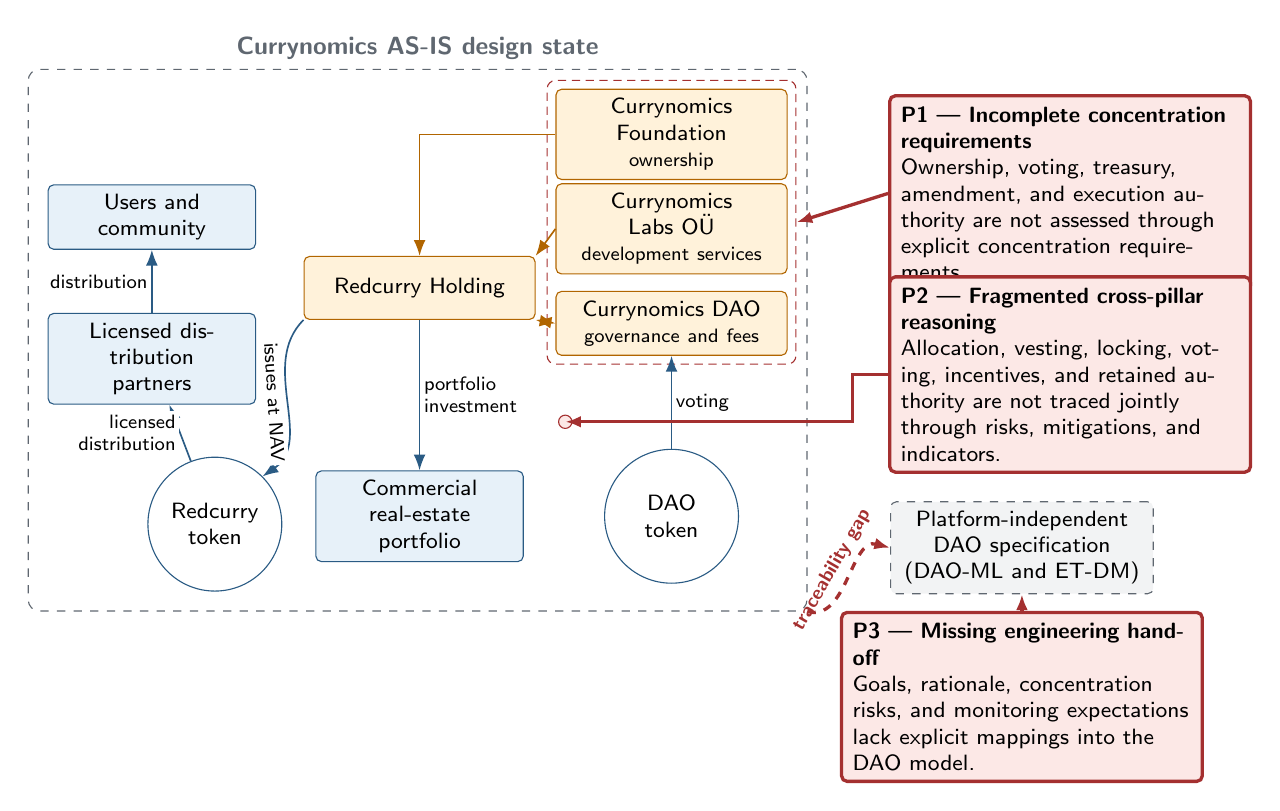
\begin{tikzpicture}[
  font=\sffamily\footnotesize,
  actor/.style={draw=asblue, fill=asbluefill, rounded corners=2pt,
    align=center, minimum height=8mm, text width=24mm},
  authority/.style={draw=asorange, fill=asorangefill, rounded corners=2pt,
    align=center, minimum height=8mm, text width=27mm},
  token/.style={draw=asblue, fill=white, circle, align=center,
    minimum size=17mm, inner sep=1.5pt},
  external/.style={draw=asgray, fill=asgrayfill, dashed, rounded corners=2pt,
    align=center, minimum height=11mm, text width=31mm},
  problem/.style={draw=asred, fill=asredfill, very thick, rounded corners=2pt,
    align=left, text width=43mm, inner sep=4pt},
  edgelabel/.style={fill=white, inner sep=1.3pt,
    font=\sffamily\scriptsize, text=black},
  flow/.style={-{Latex[length=2mm]}, semithick, draw=asblue},
  control/.style={-{Latex[length=2mm]}, semithick, draw=asorange},
  exchange/.style={<->, >=Latex, semithick, draw=asorange},
  problemline/.style={-{Latex[length=2mm]}, very thick, draw=asred},
  missing/.style={-{Latex[length=2mm]}, very thick, draw=asred, dashed}
]

\node[actor] (users) at (-5.1,1.45) {Users and\\community};
\node[actor] (partners) at (-5.1,-0.35) {Licensed distribution\\partners};
\node[authority] (holding) at (-1.7,0.55) {Redcurry Holding};
\node[authority] (foundation) at (1.5,2.50)
  {Currynomics Foundation\\{\scriptsize ownership}};
\node[authority] (labs) at (1.5,1.30)
  {Currynomics Labs OÜ\\{\scriptsize development services}};
\node[authority] (dao) at (1.5,0.10)
  {Currynomics DAO\\{\scriptsize governance and fees}};
\node[actor] (portfolio) at (-1.7,-2.35) {Commercial real-estate\\portfolio};
\node[token] (redtoken) at (-4.3,-2.45) {Redcurry\\token};
\node[token] (daotoken) at (1.5,-2.35) {DAO\\token};

\draw[flow] (partners) -- node[edgelabel,left] {distribution} (users);
\draw[flow] (redtoken) --
  node[edgelabel,left, align=right] {licensed\\distribution} (partners);
\draw[flow] (holding.south west) to[out=225,in=35]
  node[edgelabel,below,sloped] {issues at NAV} (redtoken.north east);
\draw[flow] (holding.south) --
  node[edgelabel,right,align=left] {portfolio\\investment} (portfolio.north);

% Relation meanings are stated inside the authority boxes; label-free tracks
% keep the compact diagram legible and prevent arrows from covering text.
\coordinate (ownershipturn) at (-0.25,2.50);
\draw[control] (foundation.west) -- (ownershipturn) -| (holding.north);
\draw[control] (labs.west) -- (holding.north east);
\draw[exchange] (dao.west) -- (holding.south east);
\draw[flow] (daotoken) -- node[edgelabel,right] {voting} (dao);

\begin{scope}[on background layer]
  \node[draw=asgray, dashed, rounded corners=4pt, inner sep=7pt,
    fit=(users)(partners)(holding)(foundation)(labs)(dao)(portfolio)(redtoken)(daotoken),
    label={[font=\sffamily\bfseries\small, text=asgray]above:
      Currynomics AS-IS design state}] (boundary) {};
\end{scope}

\node[problem, anchor=west] (p1) at (4.25,1.75)
  {\textbf{P1 --- Incomplete concentration requirements}\\
   Ownership, voting, treasury, amendment, and execution authority are not
   assessed through explicit concentration requirements.};
\node[problem, anchor=west] (p2) at (4.25,-0.55)
  {\textbf{P2 --- Fragmented cross-pillar reasoning}\\
   Allocation, vesting, locking, voting, incentives, and retained authority
   are not traced jointly through risks, mitigations, and indicators.};
\node[external] (model) at (5.95,-2.75)
  {Platform-independent\\DAO specification\\(DAO-ML and ET-DM)};
\node[problem, anchor=north] (p3) at (5.95,-3.55)
  {\textbf{P3 --- Missing engineering handoff}\\
   Goals, rationale, concentration risks, and monitoring expectations lack
   explicit mappings into the DAO model.};

% Each diagnosis receives its own unobstructed anchor.
\begin{scope}[on background layer]
  \node[draw=asred, densely dashed, rounded corners=3pt, inner sep=3pt,
    fit=(foundation)(labs)(dao)] (authorityrisk) {};
\end{scope}
\coordinate (coupling) at (0.15,-1.15);
\node[draw=asred, fill=asredfill, circle, inner sep=1.7pt] at (coupling) {};
\draw[problemline] (p1.west) -- (authorityrisk.east);
\draw[problemline] (p2.west) -- ++(-0.45,0) |- (coupling);
\draw[missing] (boundary.south east) to[out=-15,in=165]
  node[above, sloped, text=asred, font=\sffamily\scriptsize\bfseries]
  {traceability gap} (model.west);
\draw[problemline] (p3.north) -- (model.south);

\end{tikzpicture}
}
\caption{Currynomics AS-IS state. Solid arrows summarize principal value,
service, participation, and authority relations; red callouts locate the three
problems transformed in Sections~\ref{sec:requirements}--\ref{sec:engineering}.}
\label{fig:currynomics}
\end{figure*}

The original design established important constraints and candidate choices.
Asset backing and regulated distribution leave some responsibilities with
Redcurry Holding, licensed partners, and foundation or investment actors,
whereas the DAO can participate in treasury, process, upgrade, and token-policy
decisions. Redcurry uses collateral-constrained issuance through licensed
partners. The DAO-token design combines capped supply, early allocations,
ecosystem distribution, vesting, and governance locking, while a time-sensitive
voting family was considered to balance participation and commitment. These
choices make Currynomics suitable for examining concentration because economic,
legal, incentive, and governance constraints cannot be treated independently.

In this paper, \emph{AS-IS} denotes the case design knowledge available before
application of the concentration-aware revision; it does not imply a fully
deployed operational baseline. This AS-IS state contains three connected
problems.

\begin{description}
  \item[P1: Incomplete concentration requirements.] The decentralization goal
  is not decomposed into explicit requirements that distinguish ownership,
  effective voting power, latent control capacity, and exercised control.
  Decision rights retained by regulated or operational actors are not assessed
  together with token-mediated proposal, voting, treasury, amendment, and
  execution rights.

  \item[P2: Fragmented cross-pillar reasoning.] Incentive, governance, and
  token-policy choices are recorded, but their combined concentration pathways
  are not traced systematically. Early allocations, vesting, locking,
  time-sensitive voting, participation incentives, and retained administrative
  authority may reinforce one another, yet the AS-IS design has no integrated
  risk register connecting these interactions to mitigations, indicators, and
  residual uncertainty.

  \item[P3: Missing engineering handoff.] The rationale connecting stakeholder
  goals to token and governance choices is not transferred through explicit
  mappings into platform-independent DAO-engineering specifications. Important
  assumptions about authority, concentration risk, mitigation, and monitoring
  may therefore be lost between early design and formal DAO modeling.
\end{description}

Each answer section takes a paired input from the research architecture and the
running case: Section~3 takes RQ1 and P1, Section~4 takes RQ2 and P2, and
Section~5 takes RQ3 and P3. The three resulting transformations are integrated
in the TO-BE state evaluated in Section~6.
Table~\ref{tab:case-transformation} maps each paired input to its transformation
and intended result. The TO-BE state is not a claim that Currynomics will remain
decentralized. It is a design state in which the intended distribution of
control, its risks, and its engineering implications are explicit and
reviewable.

\begin{table}[!t]
\caption{Running-case transformation across the answer sections}
\label{tab:case-transformation}
\centering
\begin{tabularx}{\linewidth}{@{}p{.16\linewidth}X X@{}}
\toprule
Paired input & Transformation & Intended TO-BE result \\
\midrule
RQ1 + P1 & Section~\ref{sec:requirements} derives concentration-aware
requirements. & Explicit requirements covering control dimensions,
decision rights, dynamics, and indicators. \\
RQ2 + P2 & Section~\ref{sec:tedm} operationalizes the requirements as TEDM
elements. & Linked activities and outputs, including a cross-pillar
concentration-risk register. \\
RQ3 + P3 & Section~\ref{sec:engineering} defines the required mappings. &
A traceable handoff into platform-independent DAO specifications,
illustrated with DAO-ML and ET-DM. \\
\bottomrule
\end{tabularx}
\end{table}
\FloatBarrier

Section~\ref{sec:evaluation} evaluates this combined TO-BE artifact rather than
treating any one transformation as sufficient. Currynomics can demonstrate
early-stage design reasoning, but its partly pre-operational status prevents it
from establishing long-term governance or economic outcomes. The operating
Uniswap and Curve Finance cases provide a complementary retrospective view of
observable governance concentration.

The operational status changed after the design-stage evidence was collected,
but the public record supports only a limited rollout. The TEDM source states
that Currynomics had not launched when the formative evaluation was conducted
~\cite{Kivilo2026Designing}. A later official update, dated 1 June 2025,
describes Redcurry as audited and deployed on Plume Mainnet, with the first
fixed-term rollout phase open to qualified participants while a retail launch
remained forthcoming~\cite{RedCurry2025Rollout}. Current official pages still
advertise early access and a pre-sale rather than a completed retail release;
the homepage also retains the older statement that the product is live on a
Polygon testnet~\cite{RedCurry2026Homepage,RedCurry2026Presale}. The Estonian
business register continued to list Currynomics Labs OÜ as registered when
accessed on 26 September 2026, but also recorded unfiled 2024 and 2025 annual
reports and a published deletion notice~\cite{EstonianBusinessRegister2026}.
Taken together, these sources justify classifying the case as a restricted,
partly operational rollout rather than either an unchanged pre-launch design
or a fully operating retail and DAO-governed ecosystem. They do not establish
a completed governance-token generation event, active DAO voting, or mature
governance and economic outcomes.

The public evidence is sufficient for a bounded AS-IS baseline. It comprises
the published stakeholder and system map; case instantiations across
incentives, governance, and tokenomics; allocation and vesting design choices;
the demonstration conducted with two Currynomics representatives; and the
aggregate evaluation involving three external experts
~\cite{Kivilo2023TokenEconomy,Kivilo2026Designing}. The thesis is publicly
licensed for reproduction and publication, but its interview appendix lists
only participant descriptors, recording dates, and audio filenames; it does
not publish the recordings, transcripts, or MAXQDA project. A public-source
audit conducted on 26 September 2026 likewise identified no public DAO voting
history or repository containing the case-internal requirements, raw
interviews, or coding material. Those non-public materials are therefore not
assumed to be discloseable or available.

Section~\ref{subsec:problem-analysis} indexes the usable public case statements
as CE1--CE5. Those records ground P1 because they specify actors, governance
scope, retained authority, hybrid decision processes, and token and voting
choices without explicit concentration requirements. They ground P2 because
the choices were documented in separate design components without a shared
cross-pillar causal-risk register. P3 uses the absence of an explicit mapping
from those design decisions and their rationale into platform-independent
DAO-ML or ET-DM specifications as the AS-IS handoff baseline. This is an
artifact-level gap, not evidence of an operational failure. Section~6 must
therefore compare the TO-BE artifact with this published design baseline and
must not claim validation against deployed DAO behavior.

\subsection{Background Literature}\label{subsec:background-literature}

The following background defines the constructs needed to interpret the
running case and the subsequent transformations. It does not repeat the gap
argument from Section~\ref{sec:introduction}. Instead, its four parts provide
the conceptual vocabulary for the remainder of the paper: token-mediated DAO
governance and concentration support the treatment of P1/RQ1 in
Section~\ref{sec:requirements}; token-economy design and token engineering
support P2/RQ2 in Section~\ref{sec:tedm}; DAO engineering and traceability
support P3/RQ3 in Section~\ref{sec:engineering}; and design-science development
and evaluation provide the basis for Section~\ref{sec:evaluation}.

\subsubsection{Token-Mediated DAO Governance}\label{subsec:dao-governance}

For this study, a DAO is a token-mediated sociotechnical organization in which
participants coordinate toward shared goals through a configurable combination
of on-chain rules, off-chain processes, and distributed decision rights.
Tokens may provide membership, access, economic claims, or governance rights
and may support conditional value storage and transfer essential to DAO
operations~\cite{rikken2023ins,qin2022web3,wang2019decentralized}. The relevant
unit of analysis is therefore not either Currynomics token in isolation but the
configuration linking stakeholders, desired behaviors, decision rights,
issuance and distribution policies, and execution mechanisms.

DAO governance can be formally open while effective control remains
concentrated. Distribution-based indicators such as Gini,
Herfindahl--Hirschman, top-$k$ share, and Nakamoto-style coefficients capture
important aspects of token or voting-power concentration, but none provides a
complete account of governance~\cite{Fritsch2024VotingPower,
Han2026DAOGovernance}. Effective control also depends on turnout, delegation,
proposer eligibility, agenda control, emergency powers, contract-upgrade
privileges, and treasury execution. We therefore distinguish
\emph{ownership concentration}, \emph{effective voting-power concentration}
after turnout and delegation, \emph{latent control capacity}, and
\emph{exercised control}.

Recent evidence supports this multidimensional view. Contributor networks and
token movements shortly before proposals reveal influence that static holder
snapshots miss~\cite{Kitzler2025Governance}; institutional actors and contracts
can hold influential positions across protocols
~\cite{Eisermann2025Concentration}; and delegates or specialist risk teams can
become intermediaries without being the largest token holders
~\cite{Feulner2025Beyond}. Evidence across 570 DAOs further associates greater
voting-power concentration with weaker platform growth, conditional on factors
including scale, liquidity, staking, and long-term commitment
~\cite{Han2026DAOGovernance}. These distinctions provide the vocabulary for P1
and the evaluation criteria used later.

\subsubsection{Token-Economy Design and Token Engineering}\label{subsec:design-engineering}

Token-economy design spans three causally interdependent dimensions.
\emph{Incentives} concern rewards and penalties intended to shape behavior
toward system goals. \emph{Governance} concerns how proposal, deliberation,
voting, execution, and accountability rights are allocated. \emph{Tokenomics}
specifies issuance, distribution, allocation, transfer, value capture, and
supply-management rules~\cite{Benedetti2023}. Staking illustrates their
interaction: one mechanism can reward participation, reduce circulating
supply, and reallocate voting power. Concentration awareness therefore requires
cross-pillar reasoning rather than a separate decentralization checklist.

Kivilo's master's thesis established the direct antecedent for this integrated
view by developing a practical, stepwise token-economy design model across
incentives, governance, and tokenomics~\cite{Kivilo2023TokenEconomy}. Following
DSR, it synthesized literature into a non-algorithmic method, demonstrated the
artifact with Currynomics, and evaluated it through case-participant and expert
interviews. Its design sequence begins with stakeholders, system functions, and
desired behaviors; proceeds through incentive and governance choices; and then
addresses issuance, allocation, distribution, value, vesting, staking, and
supply-management decisions. The present TEDM retains this design lineage and
the three-pillar structure. Its extension is to add explicit concentration
requirements, cross-pillar risk reasoning, and a traceable handoff to DAO
engineering. Kivilo's model is therefore the foundation of the retained method,
not a separate competing contribution.

Quantitative token-engineering frameworks provide complementary mechanism taxonomies,
agent-based or dynamical simulation, parameter analysis, and state-space
exploration~\cite{liang2023cadcad,Sadykhov2025DeTEcT,
RiceZargham2019TokenEngineeringIII,Zargham2018StateSpaceBlockchain,
Zargham2020}. TEDM is complementary. It structures the upstream elicitation of
stakeholder goals, causal assumptions, decision rights, risks, and candidate
policies that quantitative approaches can subsequently formalize and test.
This distinction explains why resolving P2 requires both a qualitative
cross-pillar method and measurable expectations for later analysis.

\subsubsection{DAO Engineering and Traceability}\label{subsec:dao-engineering}

We use \emph{DAO engineering} to denote the disciplined progression from
organizational goals and requirements to governance and token-economy
specifications and, ultimately, implementable mechanisms. TEDM addresses the
upstream design-reasoning stage; it does not replace formal modeling,
simulation, smart-contract engineering, security analysis, or operational
monitoring.

Avanzo's DAO-engineering work provides the relevant downstream modeling
capability. DAO-ML represents organizational structures, roles, and permission
assignments. Extended Trusted DApp Modeling (ET-DM), also developed by Avanzo,
represents requirements concerning coordination, tokenized resources, voting
protocols, and execution; DAOMod integrates the complementary languages within
a DAO-development method
~\cite{Avanzo2024DAOML,Avanzo2025ExtendingTDM,Avanzo2026DAOMod}. Hereafter,
\emph{ET-DM} refers only to Avanzo's Extended Trusted DApp Modeling and must not
be confused with Kivilo's token-economy design model or with the TEDM artifact
developed in this paper. DAO-ML tool
support can further translate selected models toward smart-contract
implementations~\cite{Avanzo2025DAOMLToSolidity}. Resolving P3 therefore
requires mappings that preserve the rationale from TEDM outputs without
turning TEDM itself into a complete development lifecycle.

\subsubsection{Design-Science Development and Evaluation}\label{subsec:research-method}

Design Science Research (DSR) is appropriate because TEDM is an artifact
intended to address a practical sociotechnical design problem
~\cite{designResearch04}. The knowledge base combines token-economy frameworks,
governance and concentration research, DAO-engineering methods, and case
evidence. Concepts and decision points are synthesized into requirements and
method elements, applied to documented cases, and evaluated against their
intended analytical purpose. Following FEDS, the revision uses an artificial,
formative strategy comprising criteria-based analysis and documentary
demonstration~\cite{Venable2016}. Artifact evaluation must consequently examine
evidential traceability, internal consistency, documentary applicability,
concentration sensitivity, and representational coverage rather than claim
practitioner usability or that using the method itself causes decentralized
outcomes~\cite{Prat2015,vanPelt2021}.

Figure~\ref{fig:dsr} summarizes the development and evaluation cycle used for
the original TEDM and retained for the concentration-aware revision.

\begin{figure}[t]
  \centering
  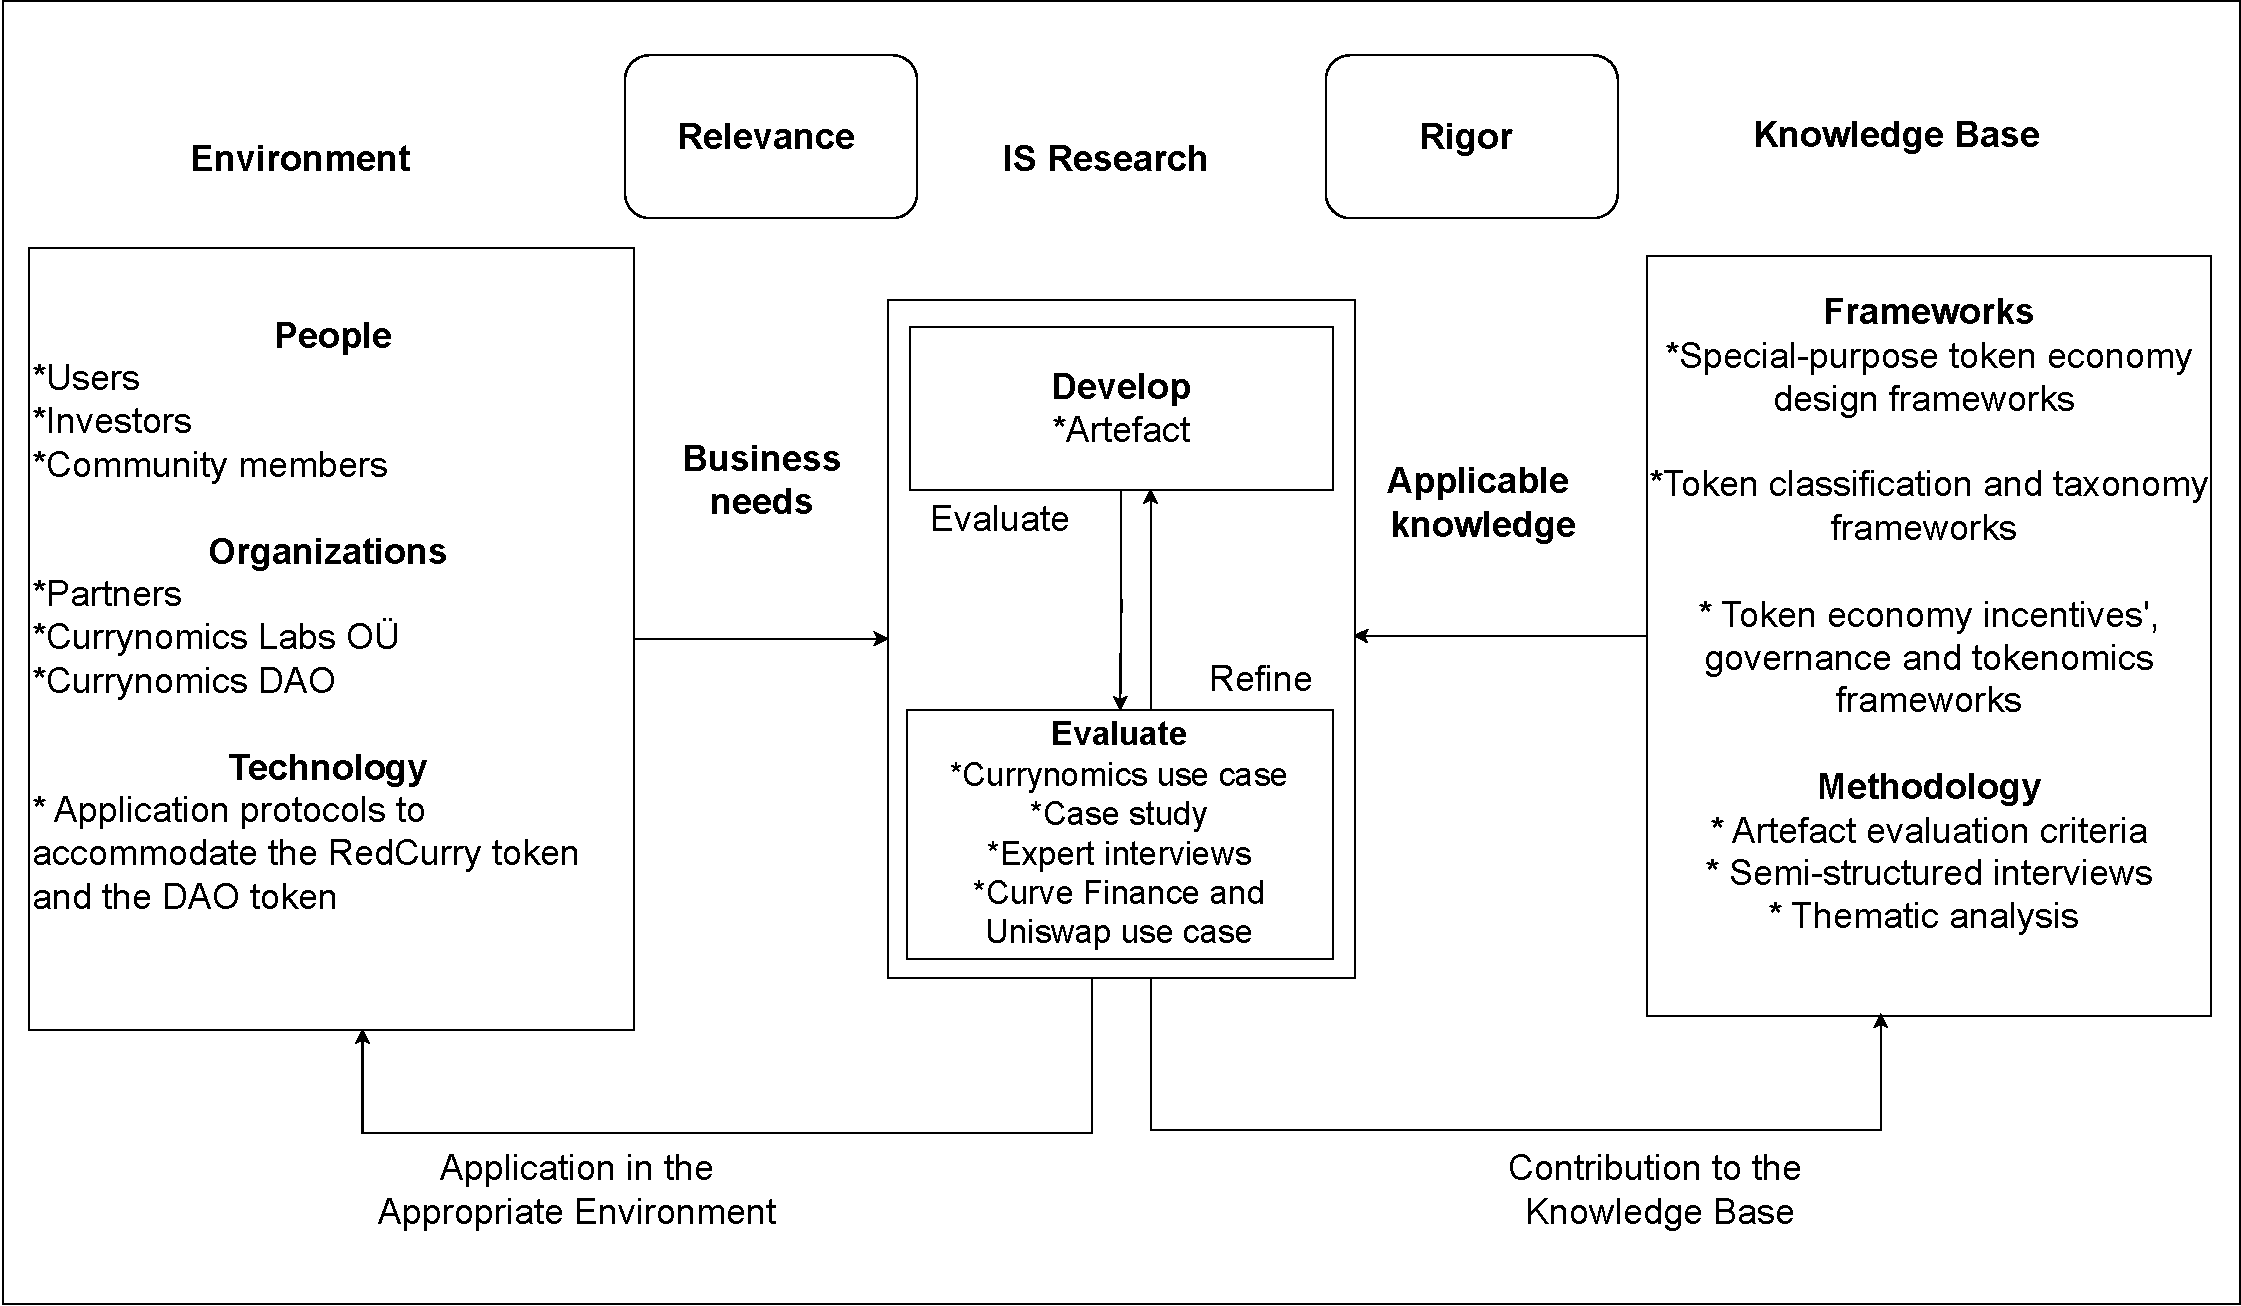
\includegraphics[width=.72\linewidth]{Token Economy Design-DSR_V2.pdf}
  \caption{Design-science cycle for developing and evaluating TEDM}
  \label{fig:dsr}
\end{figure}

Kivilo's original DSR cycle and its evidence inform the retained TEDM elements,
but that evidence cannot by itself evaluate P1--P3 or the combined TO-BE
artifact. Section~\ref{sec:evaluation} therefore separates retained evidence
about the original design model from the documentary evaluation of the new
requirements, risk register, and engineering mappings.

% ============================================================================
% SECTION 3 -- TARGET: 1,100 WORDS
% Develops the requirement profile evaluated in Section 6 and synthesized into
% the answer to RQ1 in Section 7.
% ============================================================================
\section{Requirements for Concentration-Aware Token-Economy Design}\label{sec:requirements}

Governance concentration in a DAO is not adequately characterized by token
ownership or open voting alone~\cite{Fritsch2024VotingPower,Eisermann2025Concentration,
Kitzler2025Governance}. Blockchain-governance research likewise treats
governance as the allocation and enactment of decision rights across social,
technical, and institutional layers rather than only the final vote
~\cite{vanPelt2021}. Role- and committee-based architectures may distribute
responsibilities while still assigning consequential authority to specialized
components~\cite{Jungnickel2026ModularDAO}. A design method
that leaves these pathways implicit can therefore reproduce concentrated
control even when decentralization is an explicit goal. RQ1 and the
running-case problem P1, established in Section~\ref{sec:foundations}, motivate
the need for an explicit and multidimensional requirement profile that exposes
such pathways before mechanisms are selected or transferred into engineering.

The argument proceeds in three stages. Subsection~\ref{subsec:req-motivation}
recovers the relevant knowledge from the original TEDM and relates it to
research on DAO-governance concentration. Subsection~\ref{subsec:problem-analysis}
then re-examines the retained Currynomics material to identify unresolved
concentration questions. Subsection~\ref{subsec:design-requirements} translates
the combined case and literature evidence into seven requirements with
observable satisfaction conditions. The resulting requirement profile is then
operationalized in Section~\ref{sec:tedm}, evaluated in
Section~\ref{sec:evaluation}, and used to formulate the answer to RQ1 in the
conclusion.

\subsection{Motivation and Focused Related Work}\label{subsec:req-motivation}

The original design model provides reusable knowledge that should not be
discarded. It starts by identifying stakeholders, system functions, and desired
behaviors; then considers incentive mechanisms, governance areas and roles,
the intended decentralization level, on- and off-chain processes, voting
properties, supply, issuance timing, distribution, value capture, and price
management~\cite{Kivilo2023TokenEconomy}. These elements remain the design
surface on which a concentration-aware extension must operate. Their former
organization as separate incentive, governance, and tokenomics components,
however, did not require an explicit account of how choices interact to
concentrate control.

Research on DAO governance makes those interactions visible. Token-weighted
voting can concentrate effective power among a small number of holders
~\cite{Fritsch2024VotingPower}. Time commitment can supplement token weight
and, under stated opportunity-cost or liquidity assumptions, constrain
strategic large holders~\cite{Mohan2022,Han2026DAOGovernance}. Delegation can
reduce an individual holder's information burden but may shift influence to a
smaller delegate set~\cite{Buterin2021,Han2025Review}. Airdrops can widen
initial token distribution~\cite{Lommers2023,Allen2024Airdrops}, but distribution alone does not
establish informed or sustained governance participation
~\cite{Fritsch2024VotingPower,Kitzler2025Governance}. Voting safeguards can
mitigate specified whale or collusion risks while introducing
mechanism-specific assumptions and trade-offs
~\cite{Tamai2024WhaleCollusion}. Modular DAO structures can distribute
responsibilities across components and roles, but those allocations must still
be examined for concentrated agenda-setting, emergency, or execution
authority~\cite{Jungnickel2026ModularDAO}. RQ1
therefore requires design requirements that retain the original method's useful
decision points while making their concentration implications explicit.

\subsection{Design Problem Analysis and Retained Case Evidence}\label{subsec:problem-analysis}

The former Currynomics analysis contains case material relevant to P1. It
identified stakeholder groups and system functions, distinguished community
governance from legally or operationally retained authority, and recorded
candidate allocation, locking, and voting choices. Table~\ref{tab:legacy-p1}
recasts that material as design evidence and exposes the questions that the
original analysis left unresolved. These statements describe the earlier
design state; they are not treated as evidence of deployed behavior.

\begin{table}[!b]
\caption{Legacy Currynomics design material retained for the P1 analysis}
\label{tab:legacy-p1}
\centering
\small
\begin{tabularx}{\linewidth}{@{}p{.20\linewidth}X X@{}}
\toprule
Evidence and legacy element & Retained design content & Concentration implication or open question \\
\midrule
CE1: Stakeholders and functions & Users, licensed partners, Labs, community members,
investors, Holding, and the two tokens were connected to economic and governance
functions~\citep[pp.~28--30, 34--35]{Kivilo2023TokenEconomy}. & Overlapping roles and the authority exercised by each actor require
explicit mapping. \\
CE2: Governance scope & Treasury, governance processes, protocol upgrades, and token
policy were identified as governance areas~\citep[pp.~47--48]{Kivilo2023TokenEconomy}. & Proposal, deliberation, voting,
delegation, veto, execution, and accountability rights remain incompletely allocated. \\
CE3: Retained authority & Redcurry issuance was operated by code, reserve-asset
composition was controlled by a professional investment board, and users did not
control the composition of the Currynomics Foundation board
~\citep[pp.~50--51]{Kivilo2023TokenEconomy}. & Necessary legal or operational centralization must be distinguished from
unexamined latent control capacity. \\
CE4: Hybrid process & An off-chain community-forum temperature check filtered
proposals before a key member advanced them to a formal Snapshot vote
~\citep[pp.~52--53]{Kivilo2023TokenEconomy}. & Agenda control may be concentrated even when voting is open. \\
CE5: Token and voting choices & Pre-launch DAO-token allocations, ecosystem
incentive and reserve allocations, vesting, and conviction voting with time-weighted
locking were specified~\citep[p.~58, pp.~66--72]{Kivilo2023TokenEconomy}. & Their combined effects on ownership, effective voting power, and
control over time were not traced. \\
\bottomrule
\end{tabularx}
\end{table}

The retained choices also reveal causal pathways. Private allocation can fund
development while establishing concentrated voting rights. Transferability can
improve liquidity while enabling accumulation; concentration may emerge even
after a nominally fair launch~\cite{DelgadoFernandez2024FairLaunch}. Locking can
add time commitment and, under explicit opportunity-cost and liquidity
assumptions, constrain strategic voting by large holders
~\cite{Mohan2022,Han2026DAOGovernance}. These interactions show why
P1 cannot be resolved through an ownership metric or a final compliance check.

\subsection{Design Requirements}\label{subsec:design-requirements}

The requirements were derived in four steps. First, each unresolved case issue
in CE1--CE5 was expressed as a design deficiency rather than as evidence of
deployed failure. Second, the deficiency was matched with findings about DAO
authority, voting power, token distribution, and governance safeguards. Third,
the combined evidence was translated into an obligation for the method. Fourth,
an observable satisfaction condition was specified so that the obligation can
be evaluated. This procedure yields seven requirements:

The derivation was audited through targeted online documentary verification
completed on 26 September 2026. Eight recorded OpenAlex queries tested DAO
authority, voting-power concentration, token distribution, cross-protocol
dependencies, safeguards, indicators, and engineering traceability. For each
query, the first ten ranked metadata records were inspected, or all records
when fewer were returned, giving 69 inspected records. Crossref and publisher
records verified the publication status and metadata of nine retained scholarly
sources. Official project documents were used only for case-specific design
facts, and the engineering inspection used published specifications and two
repository states fixed by full commit identifiers.

Evidence was eligible when it directly supported, qualified, or contradicted a
derivation link; addressed an RQ1 construct; had identifiable provenance and a
stable DOI, URL, or commit; and was available by the cut-off date. Duplicates,
search-result snippets, inaccessible full texts, anonymous promotional
material, and price-only studies without a governance or control relationship
were excluded. Reviewed publications superseded preprints unless the earlier
version supplied separately used material. Contrary and limiting evidence was
retained. Verification stopped when every derivation link had supporting or
limiting evidence, each project fact had an official source, and every schema
claim was tied to a fixed repository state. This stopping rule tests the stated
derivation; it does not establish exhaustive coverage of DAO research. The
exact submitted queries, screening counts, eligibility rules, versions,
locators, checksums, and evidence--deficiency--obligation records are reported
in Supplementary Tables~S7--S11.

Consistent with document-analysis guidance, source purpose and coverage were
recorded and an undocumented property was classified as unobservable rather
than absent~\cite{Bowen2009}. The chains were then checked for traceability,
singularity, consistency, feasibility, and verifiability using established
requirements-quality guidance~\cite{ISO29148}. Section~\ref{sec:evaluation}
reports the corresponding documentary audit without treating it as practitioner
validation.

\begin{enumerate}
  \item[DR1.] \textbf{Goal and decentralization-boundary traceability.} Every
  mechanism and retained authority must be connected to a stakeholder goal,
  desired behavior, quality objective, or justified legal or operational
  constraint.
  \item[DR2.] \textbf{Material authority allocation.} The method must identify
  who holds the following material rights: propose, deliberate, vote, delegate,
  veto, execute, amend, upgrade,
  invoke emergency powers, and control treasury resources, including off-chain
  authority and implementation responsibility.
  \item[DR3.] \textbf{Multidimensional concentration analysis.} Ownership,
  effective voting power after turnout and delegation, latent control capacity,
  and exercised control must be assessed separately rather than inferred from
  token holdings alone.
  \item[DR4.] \textbf{Cross-pillar and dynamic pathway analysis.} Incentive,
  governance, and token-policy choices must be examined jointly across initial
  allocation, transfer, participation, accumulation, vesting, locking, and
  delegation over time, including material cross-protocol dependencies.
  \item[DR5.] \textbf{Mitigation and residual-risk documentation.} Every
  material concentration pathway must be connected to candidate safeguards,
  their assumptions and trade-offs, and the exposure remaining after
  mitigation.
  \item[DR6.] \textbf{Indicators and interpretation rules.} Design objectives
  and risks must be connected to prospective quantitative indicators or
  qualitative tests with stated interpretation rules, reference conditions, and
  review triggers, while acknowledging that no single measure establishes
  decentralization or capture.
  \item[DR7.] \textbf{Engineering-ready traceability.} Results must be expressed
  as traceable engineering requirements and constraints suitable for subsequent
  representation in platform-independent DAO specifications.
\end{enumerate}

RQ1 concerns requirements for an early-stage, concentration-aware token-economy
design method and its design-to-specification outputs. DR1--DR7 are neither
universal governance requirements for every DAO nor evidence that satisfying
them makes a DAO decentralized or resistant to capture. For the audit, an
authority or pathway is material when exercising, withholding, or following it
can change a goal-relevant decision or one of DR3's four concentration
dimensions. A prospective causal-pathway record must identify its source,
intermediate mechanism, affected actor and governance area, concentration
dimension, lifecycle stage, consequence, and the evidential status of each
link. Residual-risk, interpretation-rule, and destination-coverage records are
accepted only when the mandatory fields in Supplementary Table~S9 are present;
missing or ambiguous fields produce a partially observable result rather than
an inferred absence. These are audit rules for design records, not causal or
behavioral effectiveness claims.

\begin{table}[!t]
\caption{Derivation and observable evaluation conditions for DR1--DR7}
\label{tab:requirement-derivation}
\centering
\footnotesize
\begin{tabularx}{\linewidth}{@{}p{.07\linewidth}p{.39\linewidth}X@{}}
\toprule
Req. & Derivation basis & Observable satisfaction condition and evaluation focus \\
\midrule
DR1 & Our re-analysis finds that CE1 and CE3 record goals and retained authority
without linking every mechanism to a rationale~\citep{Kivilo2023TokenEconomy}.
& Every mechanism and retained authority links to a goal or documented
constraint; the documentary audit checks for missing and unsupported links. \\
DR2 & CE2--CE4 separate governance scope, retained authority, and proposal
filtering; governance frameworks distinguish decision rights, accountability,
roles, and layers~\citep{Kivilo2023TokenEconomy,vanPelt2021,
Jungnickel2026ModularDAO}. & Every enumerated material governance action has an identified
responsible actor; the documentary audit checks the enumerated rights for
uncovered actions. \\
DR3 & CE3--CE5 do not separate holdings from control, although turnout,
delegation, and privileged roles alter effective power~\citep{Fritsch2024VotingPower,
Eisermann2025Concentration,Han2026DAOGovernance}. & Ownership, effective voting
power, latent capacity, and exercised control are represented separately; case
documents are checked for distinctions and unobservable dimensions. \\
DR4 & CE5 omits interactions over time; tradability can produce post-launch
concentration and shared holdings create cross-protocol dependencies
~\citep{DelgadoFernandez2024FairLaunch,
Eisermann2025Concentration}. & Each material choice is checked across pillars,
lifecycle stages, and relevant cross-protocol dependencies, with causal
pathways documented; cross-case documentary analysis checks whether the
requirement exposes interactions omitted by single-pillar descriptions. \\
DR5 & Safeguards address defined threats, while role and committee allocations
distribute rather than eliminate authority
~\citep{Tamai2024WhaleCollusion,Jungnickel2026ModularDAO}. & Every material
pathway has a safeguard, assumptions, trade-offs, and residual risk; the audit
checks field coverage and internal consistency. \\
DR6 & Distribution metrics omit identity, participation, contributor influence,
and off-chain control and cannot alone establish decentralization
~\citep{Fritsch2024VotingPower,Kitzler2025Governance,
Eisermann2025Concentration}. & Each indicator or
qualitative test specifies its control dimension, unit or assessment basis,
identity assumption where relevant, reference condition, and review trigger;
the audit checks whether another analyst can reconstruct the interpretation
from the documented rule. \\
DR7 & Because DAO-ML and DAOMod provide downstream modeling targets, this study
requires DR1--DR6 outputs to retain their identifiers and rationale across the handoff
~\citep{Avanzo2024DAOML,Avanzo2026DAOMod}.
& Every accepted choice and residual risk has a requirement identifier and a
downstream target; schema inspection checks destination coverage and records
unsupported constructs or information loss. \\
\bottomrule
\end{tabularx}
\end{table}

Together, DR1--DR7 form a proposed design-to-engineering chain whose
documentary coverage and internal consistency are evaluated in
Section~\ref{sec:evaluation}. DR1 establishes the
rationale and justified boundaries; DR2 allocates authority; DR3 separates the
dimensions in which concentration can occur; DR4 traces how it develops across
mechanisms and time; DR5 treats the resulting risks; DR6 makes them reviewable;
and DR7 preserves the results for engineering. The requirements are designed as
complementary rather than alternative checks; the audit examines whether they
collectively maintain continuity between design intent, concentration analysis,
risk treatment, and downstream specification. Exhaustiveness across all DAO
archetypes remains a proposition for later naturalistic evaluation.

CE1 and CE3 motivate traceability and explicit authority boundaries (DR1--DR3),
while CE2 and CE4 expose decision rights outside the final vote (DR2--DR3).
CE5 makes concentration a cross-pillar and temporal concern (DR3--DR4). Once
such pathways are explicit, they require documented treatments and indicators
(DR5--DR6), and their rationale must survive transfer into DAO engineering
(DR7). Table~\ref{tab:requirement-derivation} records the derivation presented here
and the evidence by which each requirement can later be assessed.

DR1--DR7 specify \emph{what} a concentration-aware method must satisfy;
Section~\ref{sec:tedm} specifies \emph{how} its activities satisfy them. DR6
requires a prospective measurement plan rather than claiming that concentration
has already been measured. Likewise, DR7 requires an engineering-ready output
but does not prescribe its modeling constructs; those mappings are derived in
Section~\ref{sec:engineering}. The conditions in
Table~\ref{tab:requirement-derivation} define the evaluation targets used in
Section~\ref{sec:evaluation} without prejudging the evaluation results.

% ============================================================================
% SECTION 4 -- TARGET: 2,200 WORDS
% Develops the method artifact used to answer RQ2 in Section 7. Protect explanatory space:
% one claim per paragraph, examples after difficult concepts, and one overview
% figure that allows the entire method to be understood before the details.
% ============================================================================
\section{The Concentration-Aware Token Economy Design Method}\label{sec:tedm}

Token-economy choices that appear defensible in isolation can combine to
concentrate control. An allocation intended to finance development can dominate
voting; a lock intended to reward commitment can amplify that advantage; and an
open vote can remain bounded by concentrated proposal, execution, or emergency
authority. Designers therefore need more than a catalogue of mechanisms or a
decentralization check performed after implementation. They need a method that
makes these interactions reviewable while choices can still be revised. This
need motivates the concentration-aware revision of TEDM developed in this
section. It retains the original method's practical stakeholder, incentive,
governance, voting, and token-policy decisions while adding the controls needed
to address the Currynomics cross-pillar problem P2.

The argument proceeds from method rationale to executable and traceable
outputs. Section~\ref{subsec:tedm-positioning} first positions TEDM in relation
to existing qualitative and quantitative approaches, after which
Section~\ref{subsec:tedm-overview} converts Section~\ref{sec:requirements}'s
DR1--DR7 into an iterative
execution protocol. Sections~\ref{subsec:goals-functions}--
\ref{subsec:token-policy} then develop its framing, incentive, governance, and
token-policy activities using the retained Currynomics evidence. Section~
\ref{subsec:risk-register} integrates their interactions in the concentration-
risk register and monitoring plan, and Section~
\ref{subsec:tedm-reassessment} checks the revision against the retained expert
feedback. Finally, Section~\ref{subsec:method-outputs} consolidates the artifact
before its engineering transfer in Section~\ref{sec:engineering}. The answers to
the research questions are synthesized in Section~\ref{sec:conclusion}.

\subsection{Method Positioning and Scope}\label{subsec:tedm-positioning}

TEDM operationalizes the requirements from Section~\ref{sec:requirements} as
a qualitative, stepwise design method for early design reasoning. It narrows
the design space, exposes trade-offs, and produces structured inputs for later
modeling, simulation, and technical implementation. In this role, TEDM
complements quantitative token-engineering approaches: it supplies the goals,
authority allocations, assumptions, and candidate policies that those
approaches can formalize and test, but it neither searches automatically for an
optimal configuration nor prescribes quantitative parameters. The unit of
analysis is a \emph{candidate token-economy design}, not a deployed DAO. Its
outputs are therefore design propositions and testable risk hypotheses, not
predictions of post-deployment behavior. The revision retains the original
method's practical scope while adding concentration analysis and engineering
traceability.

Figure~\ref{fig:original-tedm} restores the detailed baseline artifact reported
for the original TEDM~\cite{Kivilo2023TokenEconomy,Kivilo2026Designing}. It is
retained because the revised method builds on, rather than replaces, the five
incentive, seven governance, and five token-policy steps represented there. The
figure also makes the delta introduced by the concentration-aware control flow
in Figure~\ref{fig:tedm-overview} directly inspectable.

\begin{figure}[p]
  \centering
  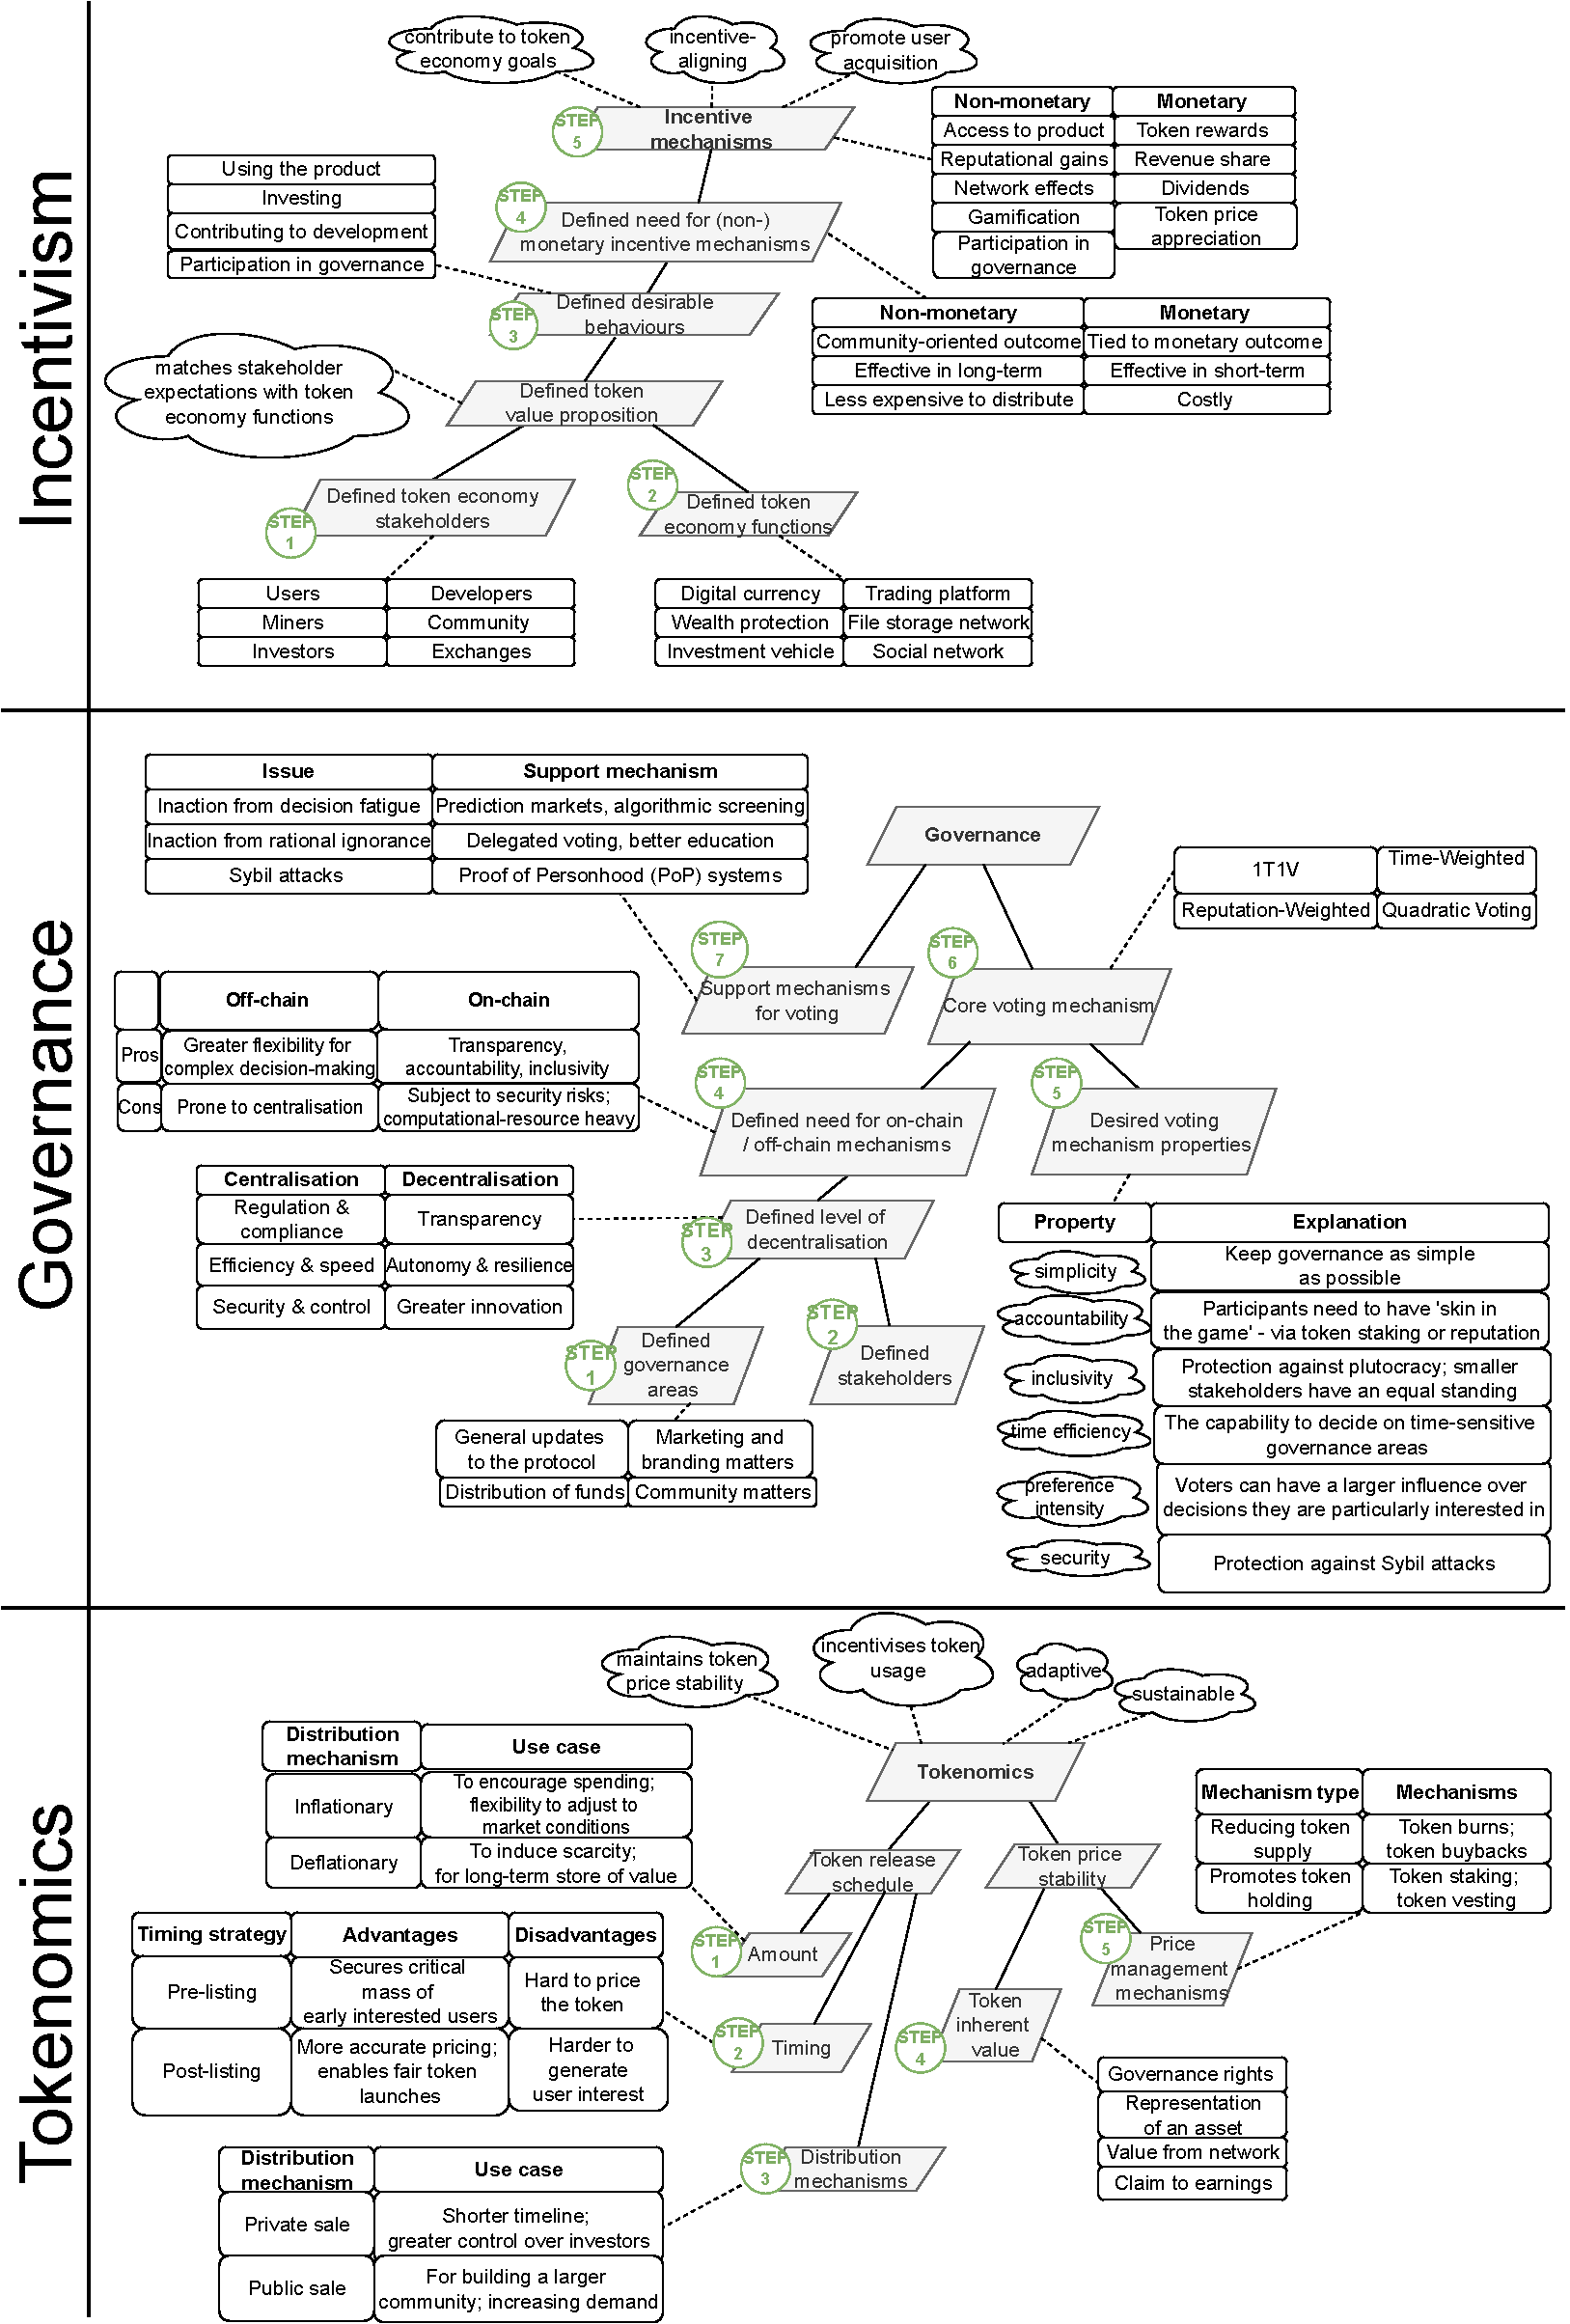
\includegraphics[width=\linewidth,height=.88\textheight,keepaspectratio]
    {Token Economy Design-Complete method image_v3.pdf}
  \caption{Original Token Economy Design Method retained as the baseline for
  the concentration-aware revision}
  \label{fig:original-tedm}
\end{figure}

\subsection{Method Overview}\label{subsec:tedm-overview}

Figure~\ref{fig:tedm-overview} retains the original five incentive, seven
governance, and five token-policy steps but replaces the former linear reading
with an explicit control flow. Decisions from the three pillars enter a
cross-pillar concentration review. Unacceptable pathways return to the relevant
pillar; accepted pathways proceed to treatment, monitoring, and the engineering
handoff.

\begin{figure}[H]
\centering
\resizebox{.98\linewidth}{!}{%
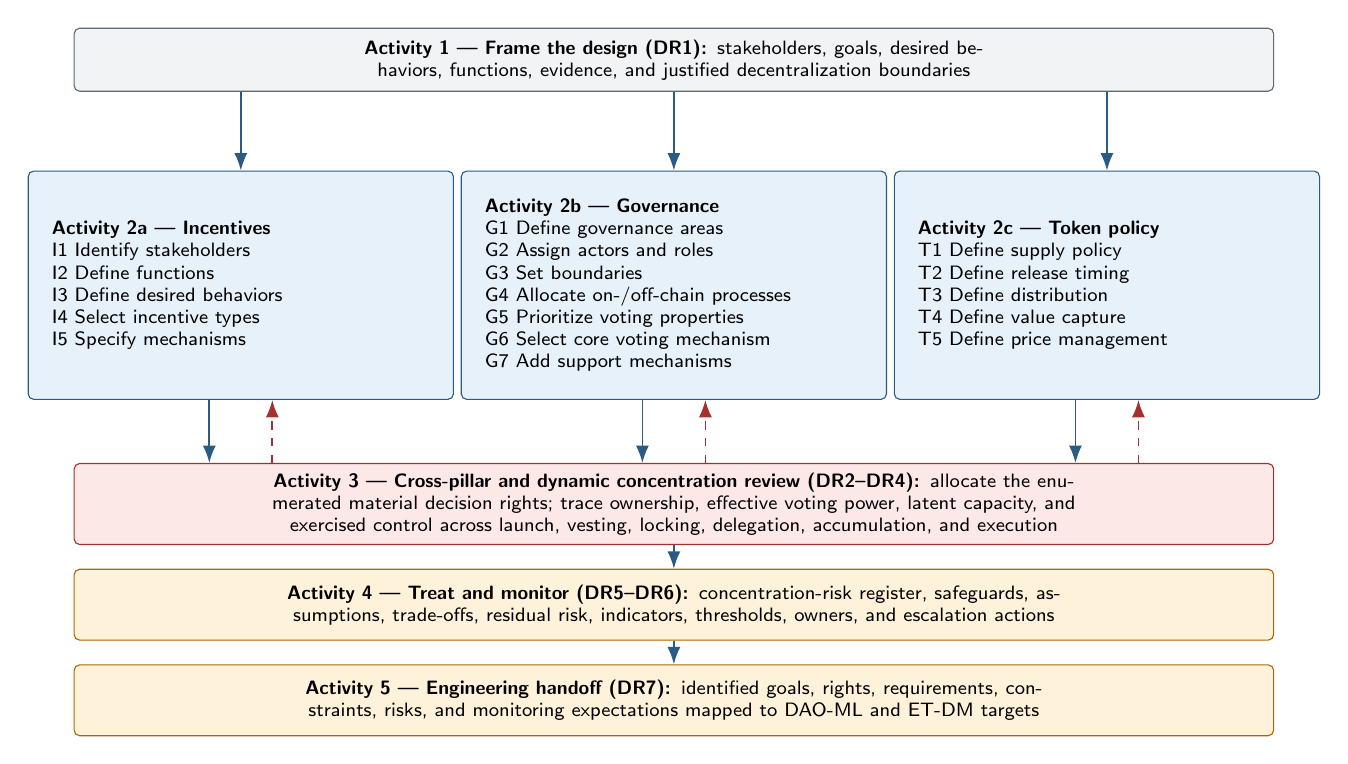
\begin{tikzpicture}[
  font=\sffamily\scriptsize,
  frame/.style={draw=asgray, fill=asgrayfill, rounded corners=2pt,
    align=center, text width=150mm, minimum height=8mm},
  pillar/.style={draw=asblue, fill=asbluefill, rounded corners=2pt,
    align=left, text width=48mm, minimum height=29mm, inner sep=3mm},
  review/.style={draw=asred, fill=asredfill, rounded corners=2pt,
    align=center, text width=150mm, minimum height=9mm},
  output/.style={draw=asorange, fill=asorangefill, rounded corners=2pt,
    align=center, text width=150mm, minimum height=9mm},
  flow/.style={-{Latex[length=2.2mm]}, semithick, draw=asblue},
  revise/.style={-{Latex[length=2.2mm]}, semithick, dashed, draw=asred}
]
\node[frame] (frame) at (0,6.4) {\textbf{Activity 1 --- Frame the design (DR1):}
stakeholders, goals, desired behaviors, functions, evidence, and justified
decentralization boundaries};
% Align the pillar tops and reserve a routing channel below Activity 1.  Using
% north anchors prevents the taller governance pillar from closing the gap.
\node[pillar, anchor=north] (inc) at
  ([xshift=-55mm,yshift=-10mm]frame.south)
{\textbf{Activity 2a --- Incentives}\\
I1 Identify stakeholders\\I2 Define functions\\I3 Define desired behaviors\\
I4 Select incentive types\\I5 Specify mechanisms};
\node[pillar, anchor=north] (gov) at ([yshift=-10mm]frame.south)
{\textbf{Activity 2b --- Governance}\\
G1 Define governance areas\\G2 Assign actors and roles\\G3 Set boundaries\\
G4 Allocate on-/off-chain processes\\G5 Prioritize voting properties\\
G6 Select core voting mechanism\\G7 Add support mechanisms};
\node[pillar, anchor=north] (tok) at
  ([xshift=55mm,yshift=-10mm]frame.south)
{\textbf{Activity 2c --- Token policy}\\
T1 Define supply policy\\T2 Define release timing\\T3 Define distribution\\
T4 Define value capture\\T5 Define price management};
% Keep a visible routing channel between the blue pillars and the review gate.
% Anchoring relative to the tallest pillar makes the gap survive text reflow.
\node[review, anchor=north] (review) at ([yshift=-8mm]gov.south)
{\textbf{Activity 3 --- Cross-pillar and
dynamic concentration review (DR2--DR4):} allocate the enumerated material decision rights;
trace ownership, effective voting power, latent capacity, and exercised control
across launch, vesting, locking, delegation, accumulation, and execution};
\node[output, anchor=north] (risk) at ([yshift=-3mm]review.south)
{\textbf{Activity 4 --- Treat and monitor
(DR5--DR6):} concentration-risk register, safeguards, assumptions, trade-offs,
residual risk, indicators, thresholds, owners, and escalation actions};
\node[output, anchor=north] (handoff) at ([yshift=-3mm]risk.south)
{\textbf{Activity 5 --- Engineering handoff
(DR7):} identified goals, rights, requirements, constraints, risks, and
monitoring expectations mapped to DAO-ML and ET-DM targets};
% Forward flow: straight, non-crossing blue arrows.
\draw[flow] ([xshift=-55mm]frame.south) -- (inc.north);
\draw[flow] (frame.south) -- (gov.north);
\draw[flow] ([xshift=55mm]frame.south) -- (tok.north);
\draw[flow] ([xshift=-4mm]inc.south) --
  ([xshift=-4mm]inc.south |- review.north);
\draw[flow] ([xshift=-4mm]gov.south) --
  ([xshift=-4mm]gov.south |- review.north);
\draw[flow] ([xshift=-4mm]tok.south) --
  ([xshift=-4mm]tok.south |- review.north);
\draw[flow] (review) -- (risk);
\draw[flow] (risk) -- (handoff);
% Revision flow: offset dashed arrows return directly to the affected pillar.
\draw[revise] ([xshift=4mm]inc.south |- review.north) --
  ([xshift=4mm]inc.south);
\draw[revise] ([xshift=4mm]gov.south |- review.north) --
  ([xshift=4mm]gov.south);
\draw[revise] ([xshift=4mm]tok.south |- review.north) --
  ([xshift=4mm]tok.south);
\end{tikzpicture}%
}
\caption{Concentration-aware TEDM. The three blue pillars retain the original
TEDM steps. Solid blue arrows show forward progression; dashed red arrows
return an unsuccessful concentration review to the affected pillar. The orange
outputs add risk treatment, monitoring, and the traceable DAO-engineering
handoff.}
\label{fig:tedm-overview}
\end{figure}

The method is executed as five activities (Table~\ref{tab:tedm-execution}).
For every material choice, designers record the selected option, rationale,
rejected alternatives, assumptions, affected stakeholders, and evidence. An
integration review then asks whether choices across pillars reinforce one
another or create a new concentration pathway. A material unresolved pathway
returns the design to the relevant activity; an acceptable but non-zero
exposure proceeds as documented residual risk. This review-and-revise gate is
the control flow added to the original step sequence.

\begin{table}[t]
\caption{Execution protocol for the concentration-aware TEDM}
\label{tab:tedm-execution}
\centering
\small
\begin{tabularx}{\linewidth}{@{}p{.19\linewidth}X X p{.13\linewidth}@{}}
\toprule
Activity & Principal decisions & Required output & DRs \\
\midrule
1. Frame the design & Stakeholders, goals, functions, desired behaviors, and
justified decentralization boundaries & Goal model and design brief & DR1 \\
2. Design the three pillars & Incentives; governance areas, rights, and voting;
supply, timing, distribution, value capture, and price policy & Three linked
decision records & DR1--DR2 \\
3. Analyze concentration & Ownership, effective voting power, latent capacity,
and exercised control across time and pillars & Causal pathways and affected
governance areas & DR3--DR4 \\
4. Treat and monitor risk & Safeguards, assumptions, trade-offs, residual risk,
and prospective interpretation rules & Concentration-risk register and
indicator plan & DR5--DR6 \\
5. Hand off to engineering & Convert accepted choices and risks into
requirements, constraints, actors, permissions, and tests & Traceability
package for DAO modeling & DR7 \\
\bottomrule
\end{tabularx}
\end{table}

\subsection{Stakeholders, Goals, and Functions}\label{subsec:goals-functions}

TEDM begins by identifying stakeholder categories and their motivations
~\cite{Khamisa2021}. Relevant categories can include maintainers, contributors,
users, token holders, developers, founders, validators, investors, regulators,
and indirect stakeholders~\cite{Davidson2021,Allen2020,Voshmgir2020,liu2022}.
One person may occupy several roles, which should be recorded because role
overlap can itself concentrate authority.

The method then identifies the functions through which the ecosystem is
expected to create value. These may include payment, investment, access,
service use, asset monitoring, collateral, or voting~\cite{Schubert2021,
Sockin2020}. For Currynomics, stakeholders include users, licensed distribution
partners, developers, community members, and investors. Redcurry is intended to
support wealth protection, investment, payment, and collateral functions,
whereas the DAO token provides participation and governance functions.

The output is a goal model linking each stakeholder to desired functions and
quality goals. It also records role overlaps and authority that must remain
centralized for legal or operational reasons. This material is retained from
the former manuscript because it provides the traceability anchor for later
mechanism choices and prevents a decentralization claim from silently expanding
beyond the authority actually delegated.

The case instantiation uses CE1--CE5 to define four stable goal/boundary records:
CG1 for asset-linked value and retained issuance/reserve authority; CG2 for
licensed access and partner authority; CG3 for bounded community governance;
and CG4 for participation without unchecked compounding of control. Their full
evidence links and downstream targets are reported in Supplementary
Table~S1. ``Retained'' authority remains subject to concentration review; it is
not presumed acceptable merely because it is legally or operationally justified.

\subsection{Incentive and Participation Design}\label{subsec:incentives}

Incentive design proceeds through five retained steps: identify stakeholders;
define token-economy functions; specify desirable behaviors; select monetary or
non-monetary incentive types; and define concrete mechanisms. Incentives should
advance system objectives, discourage destructive behavior, and account for
heterogeneous stakeholder needs~\cite{Khamisa2021,Yoo2021}. Candidate monetary
mechanisms include token rewards, staking, liquidity mining, and appreciation
expectations~\cite{Liu2022TokenIncentives}. Non-monetary mechanisms include
access, reputation, governance participation, network effects, and
gamification~\cite{Freni2022,Kim2018,liu2022}.

The concentration-aware extension adds four questions to every incentive:
Who can obtain the reward? Does the reward compound existing holdings or voting
power? Can the mechanism be exploited through multiple identities or capital
advantage? What participation pattern remains after rewards cease? In
Currynomics, Redcurry primarily uses monetary incentives linked to asset value
and stability. DAO participation was expected to rely on governance and
reputational value, with possible token appreciation as a secondary incentive.
The revised activity therefore records and tests whether participation rewards
or locking mechanisms amplify the influence of already large holders.
The activity output is an incentive decision record linking each desired
behavior to a mechanism, eligible actors, expected response, failure mode, and
concentration implication. This retains the five original steps while making
their result auditable. The Currynomics application assigns stable identifiers
to three such records: IN1 covers Redcurry's asset-value and stability
incentives; IN2 covers governance and reputational participation; and IN3
covers candidate staking rewards and their possible amplification of existing
holdings or voting power. Their complete source and risk links are reported in
Supplementary Table~S6.

\subsection{Governance and Decision-Rights Design}\label{subsec:governance-design}

The original governance component contains seven steps: define governance
areas; assign stakeholders and roles; specify the target level of
decentralization; choose on-chain and off-chain processes; define desired voting
properties; select a core voting mechanism; and add support mechanisms when
needed. Governance areas can include treasury management, process changes,
protocol upgrades, emergency action, compensation, and tokenomics
~\cite{Barrera2020,Khamisa2021}.

For every area, the revised method allocates proposal, deliberation, voting,
delegation, execution, amendment, and accountability rights. This extension is
important because an inclusive vote does not prevent concentration in agenda
setting or implementation. On-chain governance can improve transparency and
automated execution, whereas off-chain mechanisms can support deliberation and
lower transaction costs~\cite{Reijers2018}. Their combination must be
examined for authority that remains informal or technically privileged.

Candidate voting properties retained from the former manuscript are
simplicity, accountability, inclusivity, time efficiency, expression of
preference intensity, and security~\cite{Kiayas2023,Mohan2022}. The original
comparison considered 1-token-1-vote, time-weighted voting, reputation-weighted
voting, and quadratic voting. Each presents a distinct concentration trade-off:
1-token-1-vote is transparent but plutocratic; vote escrow rewards commitment
but can compound capital advantages; reputation reduces direct wealth weighting
but creates measurement and administrator power; and quadratic voting can
express intensity while requiring credible Sybil resistance.

Figure~\ref{fig:voting-matrix} retains the original comparative artifact. Its
nodes summarize literature-grounded qualitative judgments rather than measured
performance or universal rankings. Designers must therefore document why the
property priorities and mechanism assessment fit the focal governance area and
reconsider the assessment when identity, delegation, turnout, or execution
arrangements change.

\begin{figure}[t]
  \centering
  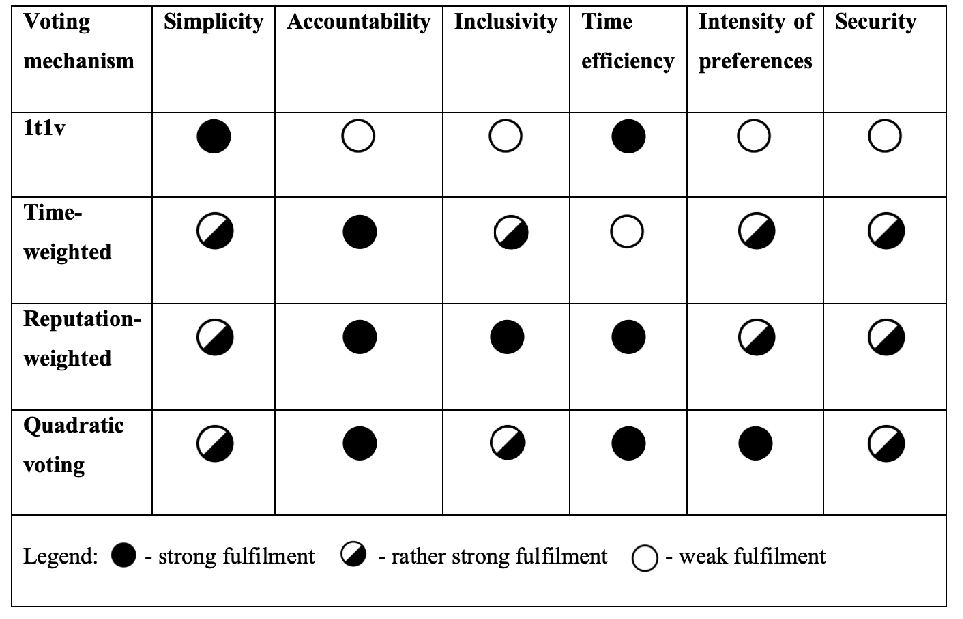
\includegraphics[width=.70\linewidth]{Table_voting_protocols_corrected.pdf}
  \caption{Retained comparison of voting-mechanism families and desired
  properties; full, half-filled, and empty nodes denote strong, partial, and
  weak expected fulfillment based on the cited literature}
  \label{fig:voting-matrix}
\end{figure}

In Currynomics, legal and operational constraints leave some decisions with an
investment or foundation board, while community participation remains possible
in treasury, process, upgrade, and token-policy areas. The original analysis
selected time-weighted conviction voting after prioritizing accountability and
security and rejecting mechanisms whose complexity exceeded anticipated needs.
The concentration-aware version must record the residual risk rather than treat
this choice as a solution to capture. The governance activity therefore ends
with a rights matrix: rows represent governance areas and lifecycle stages;
columns identify who may propose, filter, deliberate, vote, delegate, veto,
execute, amend, audit, and invoke emergency authority. Token-weighted voting is
only one cell in this wider allocation of control.

The Currynomics matrix contains five identified authority records: AR1 covers
Redcurry issuance and reserve assets; AR2 partner eligibility and distribution;
AR3 DAO treasury and parameters; AR4 governance processes and community goals;
and AR5 upgrades and DAO-token policy. Every right in Supplementary Table~S2
is allocated to an evidenced actor, identified as a proposed TO-BE control, or
left visible as an assignment gate at the level material to that governance
area. The design cannot pass Activity~3 while a material proposal, delegation,
execution, amendment, veto, emergency, audit, or accountability right remains
unassigned or lacks a justified not-applicable status.

\subsection{Token-Policy Design}\label{subsec:token-policy}

The retained tokenomics component structures five decisions: supply policy;
pre- or post-launch timing; public or private distribution; value-capture
channels; and price-management mechanisms. Supply may be capped or uncapped,
with minting and burning changing total outstanding supply over time. Capped supply
can support scarcity but encourage holding; uncapped supply can support
adaptability while creating dilution concerns. Pre-launch issuance can finance
development but produce early concentration, whereas post-launch issuance may
better follow realized demand but slow ecosystem bootstrapping.

To make the supply decision internally checkable, let $S_t$ denote total
outstanding token supply at the end of period $t$, $M_t\geq0$ authorized
minting or issuance during the period, $B_t\geq0$ verified burning or
redemption, and $S_{\max}$ an approved cap. A bounded supply transition is
\begin{equation}\label{eq:supply-transition}
S_t=\min\!\left\{S_{\max},\,
       \max\!\left\{0,S_{t-1}+M_t-B_t\right\}\right\}.
\end{equation}
The corresponding policy conditions are
\begin{equation}\label{eq:supply-conditions}
\begin{aligned}
&\text{capped:} &&0\leq S_t\leq S_{\max},\\
&\text{net inflation before the cap:} &&M_t>B_t,\\
&\text{supply-neutral:} &&M_t=B_t,\\
&\text{net deflation above zero:} &&M_t<B_t.
\end{aligned}
\end{equation}
An uncapped policy is the limiting case $S_{\max}\rightarrow\infty$. At either
boundary, Equation~\eqref{eq:supply-transition} is a bounded policy projection,
not permission to clip a proposed mint or burn silently. A quantity that would
cross a boundary must be rejected or converted into an explicitly recorded
effective amount before execution. The model is an accounting and
policy-consistency constraint, not a prediction of demand, price, or realized
circulating supply. If $C_t$ denotes the amount available for ordinary transfer,
then $0\leq C_t\leq S_t$; vesting, treasury holdings, and transfer restrictions
determine the difference $S_t-C_t$. Voting-eligible locked balances are recorded
separately because they may contribute to effective voting power without being
part of circulating supply.

Distribution through private sales, public sales, or airdrops introduces
different financing, regulatory, participation, and concentration trade-offs
~\cite{Howell2020,Gan2022,Lommers2023}. Value may be linked to governance
rights, underlying assets, network utility, or earnings~\cite{Carvalho2022,
Freni2022,Lommers2022}. Burns, staking, buybacks, and vesting may reduce
circulating supply or price shocks, but they can also create lockup cliffs,
speculative participation, or cumulative governance advantages
~\cite{Allen2022,Yoo2021}.

Redcurry uses collateral-constrained, demand-driven issuance and distribution
through licensed partners. The DAO token uses capped supply, a combination of
early allocations and later ecosystem distribution, vesting, and governance
locking. These existing design decisions remain valuable case material, but
the revised method connects them explicitly to expected voting-power
distribution and effective control. In the general case, if holder $i$ has an
eligible balance $H_{i,t}$ locked for duration $L_{i,t}$, a time-weighted rule
can be represented as
\begin{equation}\label{eq:lock-weight}
W_{i,t}=H_{i,t}f(L_{i,t}),\qquad f'(L)>0,
\end{equation}
so a longer lock produces greater voting weight for the same balance. The
chosen function, maximum duration, decay rule, and exit conditions must be
specified rather than inferred from the notation. Equation~\eqref{eq:lock-weight}
also exposes the concentration question: capital and the ability to tolerate
illiquidity can jointly determine effective voting power.

The output is a token-policy decision record with an explicit time axis
covering launch, vesting and unlock events, ordinary circulation, accumulation,
and exceptional mint, burn, redemption, or treasury actions. This time axis is
necessary because a design that appears dispersed at launch may later become
concentrated. Four identified Currynomics records make this output traceable:
TP1 covers Redcurry issuance and reserve constraints; TP2 licensed distribution;
TP3 DAO-token supply, allocation, vesting, and unlocks; and TP4 governance
locking, reward interaction, and voting-weight rules. Supplementary Table~S6
records their upstream and downstream links.

\subsection{Cross-Pillar Concentration-Risk Register}\label{subsec:risk-register}

The concentration-risk register is the principal new cross-cutting output. For
each material design choice it records the affected governance area,
stakeholders, causal pathway, expected consequence, proposed mitigation,
monitoring indicator, and residual risk. Candidate indicators include the Gini
coefficient, HHI, Nakamoto-style coefficient, top-$k$ voting share,
turnout-adjusted decisive-coalition size, delegate-network centrality,
contributor voting share, proposal-initiation concentration, pre-proposal token
flows, cross-protocol entity exposure, and treasury-signature or emergency-role
concentration~\cite{Kitzler2025Governance,Eisermann2025Concentration}.
For a non-negative distribution $x_1,\ldots,x_n$ with $\bar{x}>0$, the Gini
coefficient may be computed as
\begin{equation}
G=\frac{\sum_{i=1}^{n}\sum_{j=1}^{n}|x_i-x_j|}{2n^2\bar{x}},
\end{equation}
where higher values indicate stronger inequality. Let
$x_{(1)}\geq\cdots\geq x_{(n)}$ denote the same entity-resolved quantities in
descending order. A Nakamoto-style coefficient for majority control is
\begin{equation}
N=\min\left\{k\;\middle|\;\sum_{i=1}^{k}x_{(i)}>
\frac{1}{2}\sum_{j=1}^{n}x_j\right\},
\end{equation}
where lower values indicate that fewer independent entities can form a
controlling coalition. These measures are signals rather than proof of capture:
identities may be related, turnout may be low, delegation may alter effective
power, off-chain authority may remain invisible, and latent control may never
be exercised~\cite{Fritsch2024VotingPower}. Every proposed mitigation must
therefore record its own contingencies and residual risks. Lock-in can align
long-term incentives but entrench incumbents; delegation can widen
participation but concentrate representation; and guardians can stop attacks
while centralizing emergency authority~\cite{Han2025Review,
Han2026DAOGovernance}.

Table~\ref{tab:currynomics-risk-register} applies the register to the six
material cross-pillar pathways identified in the CE1--CE5 analysis. The four dimensions are denoted
by O (ownership), V (effective voting power), L (latent capacity), and X
(exercised control). Entries remain prospective design hypotheses, not findings
about deployed behavior; treatments are TO-BE controls to approve and test.
Supplementary Table~S3 provides the expanded auditable records, including evidence
and assumption status, affected authority, responsible owner, approval gate,
trigger and review interval, residual risk, and revision rule.

\begin{table}[p]
\caption{Case-derived concentration-risk register for the retained Currynomics design}
\label{tab:currynomics-risk-register}
\centering
\scriptsize
\begin{tabularx}{\linewidth}{@{}
>{\raggedright\arraybackslash}p{.12\linewidth}
>{\raggedright\arraybackslash}p{.13\linewidth}
>{\raggedright\arraybackslash}X
>{\raggedright\arraybackslash}X
>{\raggedright\arraybackslash}X@{}}
\toprule
ID/source & Coupled choices & Dimension, lifecycle, and pathway & TO-BE treatment &
Monitoring and residual risk \\
\midrule
CP1/CE5, TP3 & Early allocations, capped supply, vesting, and voting
rights. & O$\rightarrow$V at launch and unlocks: insiders may form a decisive
coalition before broad distribution. & Disclose entity-adjusted allocation and
vesting; stage community distribution; review every material unlock. & M1 and
M5; related wallets and secondary purchases remain uncertain. \\
CP2/CE5, IN3, TP4 & Redcurry staking rewards DAO tokens; conviction voting locks DAO
tokens for influence. & O$\rightarrow$V over participation: capital and ability
to lock can compound both rewards and durable voting power. & Simulate reward
and weighting alternatives; cap or decay amplification if the review trigger
is breached. & M1 and M6; commitment and wealth remain difficult to separate. \\
CP3/CE4, CE5 & Forum temperature check, designated proposal submission, and formal
token vote. & L$\rightarrow$X before voting: a small group can shape the agenda
of an otherwise open vote. & Publish criteria, reasons, appeals, and reviewer
activity; pluralize or rotate the filtering role. & M2; informal influence
remains partly unobservable. \\
CP4/CE3, TP1, AR1 & Code-constrained issuance, professional reserve decisions, Foundation
oversight, and technical execution. & L/X during issuance and reserve operation:
retained actors can execute, block, or redirect critical issuance and reserve
actions; separately proposed emergency controls remain prospective. & Define
mandates, separation of duties, signer thresholds, expiry, audit, and incident
disclosure. & M3 and M6; necessary legal authority remains concentrated. \\
CP5/CE1, CE3, TP2 & Licensed distribution, partner access, and market liquidity. &
O/L during distribution: a few gateways can shape access and downstream
holdings. & Diversify eligible partners subject to law; disclose exposure and
apply review limits. & M4; licensing constraints may limit feasible diversity.
\\
CP6/CE5, IN3, TP3--TP4 & Vesting, unlocks, transfers, accumulation, and later ecosystem
rewards. & O$\rightarrow$V over time: a dispersed launch can reconcentrate
through market and reward dynamics. & Maintain an entity-adjusted time series;
review before and after unlocks and large reward rounds. & M1 and M5; entity
resolution and off-market coordination remain incomplete. \\
\bottomrule
\end{tabularx}
\end{table}

The measurement plan contains six identified records: M1 measures ownership and
effective voting power; M2 agenda control; M3 privileged signer and role
coalitions; M4 partner access concentration; M5 unlock and reward dynamics; and
M6 decisive coalitions and executed control. Supplementary Table~S4 states for
each the unit, baseline, entity-resolution assumption, provisional numerical
review trigger, interval, owner, and escalation action. With no verified
operational baseline, the values are conservative review triggers to calibrate
before deployment, not decentralization certificates.

Supplementary Table~S5 reports four engineering-handoff records. ER1 carries
issuance and reserve controls; ER2 licensed distribution; ER3
proposal-to-execution authority; and ER4 allocation, vesting, rewards, locking,
and voting weight. Their source chains preserve CG, IN, AR, TP, CP, and M
identifiers and name the DAO-ML and ET-DM target classes. The supplement states
the reusable record schema immediately after Table~S6. A blank or unapproved
mandatory field remains an Activity-3 gate rather than silently omitted prose.

\subsection{Method Outputs}\label{subsec:method-outputs}

A completed application produces: a stakeholder and goal model; required system
functions and desired behaviors; selected incentive mechanisms; a governance
rights matrix; voting-property priorities and mechanism rationale; token supply,
timing, distribution, value-capture, and price-management policies; a
concentration-risk register; prospective monitoring indicators; and a set of
traceable engineering requirements. It does not produce smart contracts,
optimized economic parameters, formal security proofs, or evidence that the
implemented DAO will remain decentralized. Each output carries identifiers so
that the chain from goal to choice, risk, mitigation, indicator, engineering
requirement, and later evaluation evidence can be inspected in both directions.
For Currynomics, the documented design package comprises CG1--CG4, IN1--IN3,
AR1--AR5, TP1--TP4, CP1--CP6, M1--M6, and ER1--ER4. Its Activity-5 target column
names candidate DAO-ML and ET-DM destinations. Section~\ref{sec:engineering}
distinguishes native model constructs from information retained in the external
traceability package or treated as a possible metamodel extension.

% ============================================================================
% SECTION 5 -- TARGET: 1,000 WORDS
% Answers RQ3. Show the engineering handoff without turning the paper into a
% second paper about DAOMod or reproducing thesis material.
% ============================================================================
\section{From TEDM to DAO Engineering}\label{sec:engineering}

A concentration-aware design method has limited practical value if its results
cannot survive the transition from design reasoning to an engineering
specification. Translating only the selected token or voting mechanism is
insufficient: the resulting model may appear complete while omitting the goals,
authority boundaries, assumptions, causal pathways, mitigations, indicators,
and residual risks needed to judge whether the engineered DAO recreates an
identified prospective concentration-risk pathway. RQ3 therefore asks how the requirements derived in
Section~\ref{sec:requirements} and the method outputs produced in A2 can be transferred into
platform-independent DAO specifications without losing their rationale. P3
makes this need concrete in Currynomics, where the retained design lacks a
traceable handoff from token-economy decisions to DAO-engineering constructs.

The section develops that handoff in five steps. Section~\ref{subsec:engineering-motivation}
positions TEDM in relation to DAO engineering and identifies DAOMod as the
bounded downstream target. Section~\ref{subsec:engineering-problem} analyzes
the Currynomics handoff problem and the forms of information that may be lost.
Section~\ref{subsec:mapping} defines a type-level mapping from the material
outputs of the five A2 activities, together with their governing DR1--DR7
requirements, to DAOMod DAO-ML and ERD elements and relates it to the instance-level
records in the supplement. Section~\ref{subsec:traceability-example} then follows one
Currynomics governance decision through the proposed trace, and
Section~\ref{subsec:answer-rq3} states answer A3 and the boundary of the claimed
engineering contribution. The resulting concentration-risk handoff profile
defines the A3 target to be evaluated in Section~\ref{sec:evaluation}.

\subsection{Motivation and Related Engineering Work}\label{subsec:engineering-motivation}

TEDM was originally positioned as guidance for narrowing an extensive design
space before quantitative analysis or implementation. Expert feedback reported
in the former manuscript concerned this role and suggested technology-stack
selection and staged governance tooling as desirable extensions. Rather than
expanding TEDM into a complete development lifecycle, the revised paper defines
a bounded handoff to existing DAO-engineering work. The handoff must retain not
only the selected mechanism but also the goal, authority boundary, causal risk,
mitigation, indicator, and residual uncertainty that justify it. Otherwise, a
formally complete model may still omit the reasoning needed to review whether
the modeled DAO reproduces a concentration pathway identified during design.

This study uses DAOMod as a bounded downstream target because it combines
published platform-independent constructs for both DAO organization and
token-economy requirements, the two destinations needed by RQ3. This is a
fit-for-purpose integration target, not evidence that the mapping generalizes
to every DAO-modeling language; author overlap between TEDM and the DAOMod
publications also creates a confirmation risk addressed by fixing the audit to
public schema commits. DAOMod uses two complementary diagram types. DAO-ML
represents organizational structures, roles, and permissions; Extended Trusted
DApp Modeling (ET-DM) represents requirements concerning coordination,
tokenized resources, voting protocols, smart-contract primitives, and
on-/off-chain execution. Together
they support a stepwise method spanning the organization, coordination, and
execution layers~\cite{Avanzo2024DAOML,Avanzo2025ExtendingTDM,
Avanzo2025Thesis,Avanzo2026DAOMod}. A model-to-code route also generates Solidity roles and
permissions from DAO-ML models~\cite{Avanzo2025DAOMLToSolidity}. TEDM therefore
does not claim a new modeling language or implementation pipeline. Its proposed
contribution is a concentration-risk handoff profile: the upstream rationale,
causal assumptions, mitigations, indicators, and traceability constraints that
DAO-ML and ET-DM models should preserve. For terminological precision, the
remainder of Section~5 calls the later integrated ET-DM syntax the \emph{DAOMod
Extended Requirement Diagram (ERD) schema}; the earlier standalone ET-DM
schema is used only for version comparison.

The cited engineering lineage is used as a downstream integration target, not
as independent validation of TEDM. The documentary evaluation therefore tests
destination coverage against the published metamodels and records information
that must remain in an external traceability package. Whether independent
modelers can execute the handoff efficiently remains outside the resulting
claim.

\subsection{Design Problem Analysis and Retained Case Evidence}\label{subsec:engineering-problem}

The retained, pre-revision Currynomics material exposes the P3 handoff problem.
It recorded stakeholders, desired behaviors, governance areas, voting
properties, and token choices, but these outputs remained distributed across
diagrams, tables, and explanatory prose. They were not connected through stable
identifiers to a platform-independent model in which a reviewer could follow a
goal through a design decision to the role, permission, token rule, voting
protocol, or execution constraint that realizes it. The revised A2 artifact
addresses the upstream part of this deficiency: Activity~5 requires a
traceability package, and every method output carries identifiers through which
goals, choices, risks, mitigations, indicators, engineering requirements, and
later evaluation evidence can be linked. Section~5 must now specify where those identified outputs go and what
their DAO-model representations must preserve.

P3 concerns three forms of potential information loss. First, a design concept
may have no destination construct, leaving it unrepresented. Second, a concept
may be representable only as unstructured annotation, weakening machine or
reviewer traceability. Third, a mechanism may be modeled while its rationale,
assumptions, mitigation, or monitoring expectation is dropped. For
concentration-aware design, the third failure is especially consequential: the
same voting primitive can have different implications under different token
distributions, delegation arrangements, turnout assumptions, and retained
off-chain authority.

\subsection{Mapping TEDM Outputs to DAO Models}\label{subsec:mapping}

Table~\ref{tab:engineering-mapping} specifies the type-level handoff from the A2
output categories to DAO models and identifies the Section~\ref{sec:requirements}
requirements that govern each transfer. Supplementary Table~S5 supplies the
four engineering-requirement source chains, while Supplementary Table~S12 gives
the instance-level disposition of every CG, IN, AR, TP, CP, M, and ER identifier.
The mapping
follows three rules. Every A2 output must have a model
destination or an explicitly documented representation gap; every destination
element must retain a link to its source goal, decision record, and applicable
DR; and every material concentration pathway must remain connected to its
assumptions, mitigation, indicator interpretation rule, residual risk, and
responsible role. Bidirectional coverage and an observable verification
criterion follow established requirements-engineering guidance
~\cite{ISO29148}. These rules make Activity~5 an execution of DR7 that also
preserves the products of DR1--DR6.

The mapping is many-to-many. A governance right may require both an
organization permission and DAOMod ERD coordination and execution requirements; one quality goal
may constrain several token, voting, and organizational elements; and one risk
may connect choices from several activities. Each handoff record therefore
contains, at minimum, a source-output identifier, applicable DR, accepted choice
and rationale, relevant assumptions and rejected alternatives, destination
element identifiers, residual risk, and verification or monitoring rule.
Supplementary Table~S13 defines the fields, types, cardinalities, conditional
obligations, identifier rules, and change control of the external traceability
package; the accompanying normalized CSV schema and serialization templates are supplied with the
supplementary materials. Editable DAO-ML and ERD draw.io drafts and their
XSD-conformant semantic XML companions are also supplied as provisional review
artifacts; they instantiate candidate identifiers but are not evaluation
evidence. Supplementary Table~S9 supplies the documentary
acceptance and partial-observability rules applied to its records.
Completeness is assessed against the Section~4 output inventory and the
observable conditions for DR1--DR7. Consistency is assessed by checking that
role permissions, voting rules, token lifecycle constraints, mitigations, and
on-/off-chain execution responsibilities do not contradict one another. These
checks are applied in Section~\ref{sec:evaluation}; they establish documentary
conformance rather than independent modeler usability.

The status column separates three dimensions so proposed handoff information is
not mistaken for native metamodel support. \emph{Native coverage} is
``complete'' when the required information has dedicated schema constructs,
``partial'' when only some information is native or generic text is required,
and ``absent'' when no suitable native construct exists. \emph{Preservation
location} is ``native model'' or ``external package.'' \emph{Extension status}
is separately recorded as ``not proposed,'' ``candidate,'' ``proposed,'' or
``adopted''; candidacy is neither a storage location nor native support.
The documentary
evaluation reports construct deficits, overloaded annotations, and potential
information loss; it proposes no metamodel extension without model-construction
evidence.

The native classifications in Table~\ref{tab:engineering-mapping} were checked
against two complementary kinds of authoritative evidence. Avanzo's thesis
defines the DAOMod ontology, graphical notation, grammar, relation semantics,
XPath constraints, and method steps; the pinned DAO-ML and
ERD XSDs provide the corresponding machine-readable declarations
~\cite{Avanzo2024DAOML,Avanzo2025Thesis,Avanzo2024ETDMSchema,
Avanzo2025DAOModSchemas}. In particular, the organization notation assigns
permissions and governance areas to roles or committees through
\texttt{associated\_to}; the XSD represents that relation as \texttt{xs:IDREFS},
while the thesis supplies the endpoint-type constraint checked by XPath. Because
the earlier standalone ET-DM schema and the
later DAOMod integrated extended-requirement schema differ, the table uses the
later DAOMod ERD schema as the downstream target and identifies information that
still requires the external traceability package. All ``native,'' ``partial,''
and ``absent'' classifications are therefore bounded to the cited schema
commits, rather than asserted for every version of the modeling languages.
Supplementary Table~S14 records the exact notation rule together with the XSD
file and element, type, or attribute path supporting each classification. The earlier standalone ET-DM
schema contains specialized mechanism types that the later ERD collapses into
a generic mechanism plus an enumeration; Table~6 does not credit the later
target with constructs found only in that earlier schema.

{\footnotesize
\begin{longtable}{@{}p{.27\linewidth}p{.31\linewidth}p{.35\linewidth}@{}}
\caption{Type-level candidate representation of design requirements and A2 outputs in DAO-engineering specifications}
\label{tab:engineering-mapping}\\
\toprule
Requirement and A2 source & Candidate representation and status & Information that must survive the handoff \\
\midrule
\endfirsthead
\multicolumn{3}{@{}l}{\tablename\ \thetable\ (continued)}\\
\toprule
Requirement and A2 source & Candidate representation and status & Information that must survive the handoff \\
\midrule
\endhead
DR1; Activity~1 goal model, functions, desired behaviors, role overlaps, and justified decentralization boundaries & Coverage: partial. Native location: DAOMod DAO-ML \texttt{DAO}, \texttt{GovernanceArea}, \texttt{Role}, and \texttt{Committee}; DAOMod ERD \texttt{organizationGoal}, \texttt{goal}, \texttt{qualitygoal}, and \texttt{agent}. External location: boundary rationale. & Goal links, scope, affected stakeholders, and authority intentionally retained for legal or operational reasons \\
DR1--DR2; Activity~2 governance-rights matrix and on-/off-chain allocation & Coverage: partial. Native location: DAOMod DAO-ML \texttt{Role}, \texttt{Committee}, \texttt{Permission}, \texttt{associated\_to}, \texttt{is\_controlled\_by}, and \texttt{GovernanceArea.implementation}; DAOMod ERD \texttt{decisionMakingMethod}, \texttt{proposal}, \texttt{mechanism}, \texttt{agent}, and execution attributes. External location: distinctions among the ten TEDM rights, lifecycle stage, accountability, and informal or technically privileged authority. & Actors for proposing, deliberating, voting, delegating, vetoing, executing, amending, upgrading, invoking emergency powers, and controlling treasury resources; lifecycle stage, accountability, implementation responsibility, and informal or technically privileged authority \\
DR1--DR5; voting-property priorities, selected mechanism, rationale, and rejected alternatives & Coverage: partial. Native location: DAOMod ERD \texttt{decisionMakingMethod} with \texttt{voting\_requirement} and \texttt{proposal\_requirement}, plus \texttt{mechanism} and \texttt{qualitygoal}; DAOMod organization roles and committees. External location: rationale, rejected alternatives, and residual risk. & Property priorities, mechanism assumptions, support mechanisms, trade-offs, and residual capture risk \\
DR1, DR3--DR5; incentive decision records & Coverage: partial. Native location: DAOMod ERD \texttt{token}, \texttt{tokenManager}, \texttt{treasury}, \texttt{resource}, \texttt{mechanism}, \texttt{qualitygoal}, and \texttt{agent}. External location: expected response, failure mode, and concentration implication. & Desired behavior, eligible actors, expected response, failure mode, and concentration implication \\
DR1, DR3--DR5; token-policy record and explicit time axis & Coverage: partial. Native location: DAOMod ERD \texttt{token}, \texttt{tokenManager}, and \texttt{treasury}; \texttt{mechanism} carries \texttt{trigger}, \texttt{precondition}, \texttt{postcondition}, and \texttt{execution}. External location, with extension candidacy: lifecycle time series. & Supply and allocation rules plus launch, vesting, unlock, circulation, accumulation, and exceptional-action stages \\
DR3--DR4; causal pathways across four concentration dimensions & Coverage: absent. External location: pathway record linked to DAOMod organization roles and permissions and ERD goals, tokens, decision-making methods, and mechanisms. Extension candidate only if identifier links prove inadequate. & Ownership, effective voting power, latent capacity, and exercised control, including allocation, transfer, participation, accumulation, vesting, locking, delegation, cross-pillar and temporal effects, and material cross-protocol dependencies \\
DR5--DR6; concentration-risk register and indicator plan & Coverage: partial. Native location: DAOMod ERD \texttt{qualitygoal}, \texttt{mechanism.trigger}, and \texttt{agent}, plus DAOMod organization roles and permissions. External location: risk, indicator, baseline, review interval, and escalation records; extension candidate only after construction evidence. & Consequence, treatment, trade-off, residual risk, quantitative unit or qualitative-test basis, identity assumption, interpretation rule, reference condition or baseline, review interval, trigger, and action \\
DR7; Activity~5 engineering requirements and trace identifiers & Coverage: absent for the cross-model relation. Native models provide element identifiers; source--destination relations remain in the external package. & Source and destination identifiers, evidence references, representation gaps, bidirectional coverage, and an observable verification or acceptance criterion for each requirement \\
\botrule
\end{longtable}
}

\subsection{End-to-End Traceability Example}\label{subsec:traceability-example}

The Currynomics voting example shows how the design requirements and A2 jointly
constrain the handoff. CG4 supplies the goal of participation without unchecked
compounding of control. IN3 records candidate staking rewards; AR3 allocates the
treasury and parameter-governance rights exercised through token voting; and TP4 records locking, reward interaction, and
voting-weight rules. CP2 connects those choices to the prospective
ownership-to-effective-voting-power pathway in which capital and the ability to
lock can compound rewards and durable influence. M1 and M6 specify the ownership,
effective-power, decisive-coalition, and executed-control reviews. ER4 packages
the allocation, vesting, reward, locking, and voting-weight constraints for the
engineering handoff. The resulting source chain is
CG4 $\rightarrow$ IN3/AR3/TP4 $\rightarrow$ CP2 $\rightarrow$ M1/M6
$\rightarrow$ ER4.

The candidate model fragment assigns provisional downstream identifiers so the
trace can be tested without presenting them as evaluated case evidence.
DAO-ML elements \texttt{GA-AR3}, \texttt{ROLE-COMMUNITY},
\texttt{PERM-AR3-PROPOSE}, \texttt{PERM-AR3-FILTER},
\texttt{PERM-AR3-VOTE}, \texttt{PERM-AR3-EXECUTE},
\texttt{PERM-AR3-VETO}, \texttt{PERM-AR3-AUDIT}, and
\texttt{PERM-AR3-EMERGENCY} are candidate identifiers for the governance area,
participating role, and decomposed proposal-to-execution authority. DAOMod ERD elements
\texttt{OG-CURRYNOMICS}, \texttt{G-CG4}, \texttt{DM-ER4}, \texttt{TK-DAO},
\texttt{M-IN3-STAKING}, and \texttt{M-TP4-LOCKING} represent the organization
goal, its participation-goal refinement, decision-making method, DAO token, staking mechanism, and locking
mechanism. Quality-goal elements record the applicable accountability,
security, and inclusivity objectives. External trace record \texttt{TR-CP2}
links these native elements to CP2, M1, M6, the rejected alternatives,
mitigation rationale, residual risk, and review rules. The documentary
conformance inspection of the cited schema commits identifies the named target classes and records
representation gaps. The supplied first-draft semantic models pass the pinned
XSDs and the thesis-defined reference and hierarchy checks; independent expert
review, correction of provisional assignments and notation, and a reported
reconstruction remain necessary before they can count as evaluation evidence.

The candidate trace is therefore:
\begin{quote}
CG4 $\rightarrow$ IN3/AR3/TP4 $\rightarrow$ CP2 $\rightarrow$ M1/M6
$\rightarrow$ ER4 $\rightarrow$ \texttt{TR-CP2} $\rightarrow$
DAO-ML and DAOMod ERD elements.
\end{quote}

\FloatBarrier
\subsection{Answer to RQ3}\label{subsec:answer-rq3}

\textbf{A3.} The required traceability mappings take the DR1--DR7 requirement
profile from Section~\ref{sec:requirements} and the identified outputs of all five A2 activities as their
source. They connect goals and authority boundaries, enumerated material decision rights,
incentive and token-policy records, voting rationale, four-dimensional causal
pathways, and supported portions of mitigations to native organization,
coordination, token-economy, voting-protocol, and execution constructs in
complementary DAO-ML and DAOMod ERD models. Causal-pathway details, mitigation
trade-offs, residual risks, indicator plans, baselines, interpretation rules,
review triggers, and cross-model trace relations remain in the external
traceability package, which is normative for the proposed TEDM handoff profile,
because the inspected native syntaxes have no
complete constructs for them. Under the proposed profile, a conforming handoff
must provide bidirectional source and destination coverage, preserve rationale
and temporal dependencies, expose unsupported constructs, and permit consistency checks
across roles, token rules, voting, risk treatment, and execution. Together these
elements form a proposed concentration-risk handoff profile addressing P3 at
the specification level. Section~\ref{sec:evaluation} documents destination
coverage in the inspected schemas and identifies native representation gaps; it does not
establish independent modeler usability. Platform selection, implementation,
deployment, and behavioral verification remain responsibilities of downstream
methods and tools.

% ============================================================================
% SECTION 6 -- TARGET: 2,400 WORDS
% Evaluate the requirements, method, and engineering handoff. The final
% concentration-aware artifact must be evaluated;
% evidence gathered only for an earlier TEDM version cannot be treated as full
% documentary evaluation of the revised method.
% ============================================================================
\section{Evaluation Evidence and Independent-Use Protocol}\label{sec:evaluation}

\subsection{Evaluation Strategy and Documentary Corpus}
\label{subsec:evaluation-criteria}

The evaluation has three deliberately separate evidentiary components. First,
the five interviews reported by Kivilo provide historical, formative evidence
about the original TEDM. Second, a criteria-based documentary audit evaluates
properties of the revised artifact that can be inspected without users:
evidential traceability of DR1--DR7, requirements quality and internal
consistency, applicability to documented DAO cases, comparative diagnostic
coverage within the recoded materials, and destination coverage of the
engineering handoff. Third, the independent-use protocol specified below is
required to evaluate whether external researchers and practitioners can use
the revised method as intended. FEDS recognizes criteria-based analysis,
theoretical argument, and documentary demonstration as artificial evaluation
episodes while reserving claims about effectiveness in real use for
naturalistic evaluation~\cite{Venable2016}. The three components are therefore
not pooled: evidence about one version or one kind of evaluand is not treated as
evidence about another.

The documentary corpus has three layers. The derivation layer contains the
peer-reviewed and archival research cited in Section~\ref{sec:requirements}.
The case layer contains Kivilo's publicly available thesis for Currynomics and
official Uniswap and Curve publications available by 26 September 2026
~\cite{Kivilo2023TokenEconomy,Uniswap2020UNI,Uniswap2021V3,
CurveDAO2020,CurveDocs2026}. The representation layer contains the published
DAO-ML, ET-DM, and DAOMod specifications cited in Section~\ref{sec:engineering}.
Official project documents are used for stated mechanisms, allocations, roles,
and procedures, not as independent evidence that those arrangements are
decentralized or effective. Following document-analysis guidance, source type
and scope were distinguished for each reported observation; missing documentation is classified
as \emph{unobservable}, not as evidence of absence~\cite{Bowen2009}.

The audit applies the conditions in Table~\ref{tab:requirement-derivation} and
the characteristics of well-formed requirements---including singularity,
unambiguity, feasibility, verifiability, consistency, and traceability---used
in established requirements-engineering guidance~\cite{ISO29148}. Findings are
reported as supported, partially observable, or representational gap. This
scale avoids converting documentary coverage into a claim of universal
completeness.

\subsection{Replication Package and Evidence Status}
\label{subsec:replication-package}

The TEDM replication package is maintained separately from the institutional
knowledge-graph governance evaluation in the MKM project repository:
\url{https://github.com/alexbafana/MKM-POL21-2025/tree/3f842be/reproducibility/tedm}.
It contains the supplied documentary case-record source, candidate destination
mappings, traceability schema and serialization templates, provisional DAO-ML
and DAOMod ERD models, and an independent reconstruction protocol. The URL pins the executed audit package to commit \texttt{3f842be};
subsequent artifact corrections require a new version and citation. An archival
release identifier remains to be added after independent review.

Artifact availability is distinguished from completed evaluation. The supplied
models are author-built first drafts; the machine-readable package now serializes the supplied case tables into
32 proposed records and 159 source-explicit links. These are documentary
serializations, not new empirical observations. The independent reconstruction protocol
has not been executed. The automated audit reproduced conformance of both semantic models to the
pinned XSDs, checked diagram XML parsing, and resolved the record-link and
mapping-source identifiers. It did not reproduce the full thesis XPath suite
or establish semantic validity. Visual refinement,
schema conformance, semantic review, and independent reconstruction are separate
checks and must be reported with their actual evidence status.

The planned reconstruction uses the CG4--IN3/AR3/TP4--CP2--M1/M6--ER4 source
chain. An independent modeler receives a frozen source package and target
schema versions, but not the author-built model before submitting the initial
reconstruction. A pre-specified rubric assesses authority allocation, mechanism
semantics, trace coverage, contradictions, representation gaps, and preservation
of treatment, residual risk, and monitoring. Assistance, discrepancies,
failures, adjudication, and resulting revisions must be retained. Until those
deliverables exist, this protocol adds reproducibility instructions rather than
independent engineering evidence.

\subsection{Retained Legacy Evaluation Evidence}
\label{subsec:expert-evaluation}

Kivilo's published thesis records the original Currynomics demonstration and
five semi-structured interviews: two case participants and three external
experts with at least three years of token-economy experience. The study used
purposive sampling, transcription, and thematic analysis and assessed
completeness, simplicity, understandability, operational feasibility, and
perceived accuracy~\cite{Kivilo2023TokenEconomy,Braun2014}. Participants valued
the integrated structure and its ability to rule out unsuitable mechanisms,
while requesting clearer navigation, quantitative follow-up, legal and
game-theoretic boundaries, staged governance, distribution guidance, and a
later technical handoff. These findings motivated retained and revised TEDM
features, but they evaluate only the artifact shown in 2023. They are not
relabelled as participant validation of DR1--DR7.

The published coding summary contains 55 comment segments: completeness
(3 supportive, 4 neutral, 2 opposing), simplicity (7, 2, 0),
understandability (0, 2, 3), operational feasibility (6, 8, 0), and perceived
accuracy (4, 11, 3). These counts describe coded statements rather than
independent observations or statistical evidence. Their role in the present
evaluation is historical and formative.

Table~\ref{tab:legacy-participants} restores the participant-role information
needed to interpret that evidence. The role descriptions establish relevant
experience but do not make the two case participants independent of the focal
case or show that any participant inspected the revised control flow, risk
register, monitoring records, identifiers, or engineering handoff.

\begin{table}[t]
\caption{Participants in the retained evaluation of the original TEDM}
\label{tab:legacy-participants}
\centering
\footnotesize
\begin{tabularx}{\linewidth}{@{}p{.10\linewidth}p{.35\linewidth}X@{}}
\toprule
Code & Role & Reported background \\
\midrule
IN1 & Currynomics co-founder & Business development; MBA \\
IN2 & Currynomics co-founder & Engineering; BSc in information technology \\
IN3 & External expert & Electrical engineer and token-engineering researcher \\
IN4 & External expert & Web3 project consultant and adviser \\
IN5 & External expert & Computer scientist, developer, and Web3 infrastructure founder \\
\bottomrule
\end{tabularx}
\end{table}

\subsection{Artifact Reassessment Against the Legacy Findings}
\label{subsec:tedm-reassessment}

The legacy interviews cannot validate the concentration-aware revision, but
their negative and mixed findings provide an explicit baseline for formative
reassessment. Navigation and unfamiliar terminology are addressed by numbered
activities, stable identifiers, and a single control flow; legal boundaries by
CG1--CG4 and AR1--AR5; staged governance by separating proposal, decision,
execution, and emergency rights; quantitative follow-up by M1--M6 and the
simulation gates; dilution and cascade concerns by lifecycle reviews; and
implementation guidance by the bounded Activity-5 handoff. DAO-archetype
variation is addressed through case-specific boundaries and threshold
calibration rather than universal parameters. These are design responses to
previous findings, not participant assessments of whether the responses work.

\subsection{Independent Comparative Evaluation Protocol}
\label{subsec:independent-evaluation}

Independent evaluation of the revised artifact must use participants who did
not design TEDM and who have relevant experience in at least one of token
engineering, DAO governance, or platform-independent DAO modeling. Recruitment
should record role, years and type of experience, prior familiarity with TEDM,
and any relationship to the cases. A purposive sample should cover all three
competence areas and continue beyond an initial minimum of six participants if
the last completed round still produces a new critical omission. Case owners
may provide contextual feedback, but their assessments must be identified
separately from those of independent participants.

The study should use a counterbalanced within-participant comparison. Each
participant receives the original TEDM, the revised TEDM, matched DAO design
vignettes, the same source packet, blank record templates, and a glossary.
Case--method order is rotated across participants to reduce learning and case
effects. Without coaching from an artifact author, participants must (1)
identify actors, goals, and material decision rights; (2) select and justify
incentive, governance, and token-policy choices; (3) identify cross-pillar and
temporal concentration pathways; (4) specify mitigations, residual risks, and
monitoring rules; and (5) transfer one accepted pathway into DAO-ML and ET-DM
or mark the missing destination explicitly. Sessions should capture the
completed records, task time, clarification requests, observed breakdowns, and
a semi-structured debrief, subject to ethics approval and informed consent.

The original criteria---completeness, simplicity, understandability,
operational feasibility, and perceived accuracy---permit comparison with the
legacy study~\cite{Prat2015}. Four revision-specific criteria are added:
concentration sensitivity, traceability, internal consistency, and engineering
compatibility. Observable measures include the number and type of material
pathways found; unsupported or contradictory choices; complete
goal--choice--risk--mitigation--indicator--requirement chains; correctly
preserved identifiers; mapping ambiguities and information loss; and
participant ratings with explanations. Counts are descriptive task evidence,
not independent statistical observations.

Two analysts who were not the participant's facilitator should code the task
artifacts and interview material against a versioned codebook. They should code
an initial subset independently, discuss disagreement, revise the codebook,
then retain an audit trail of final judgments. Analysis must report divergent
cases, failed tasks, requests for assistance, and findings that favor the
original method, not only improvements under the revision. A revision log must
connect each accepted finding to the affected figure, field, instruction, or
mapping; rejected suggestions require a recorded rationale.

This protocol had not been executed at the reporting date. Consequently, this
article contains no new participant result for DR1--DR7, the revised Figure~3
control flow, CP1--CP6, M1--M6, the identifier scheme, or the DAO-ML/ET-DM
handoff. Until those data are collected, the defensible findings are limited to
the legacy evidence and the documentary results reported next; practitioner
understandability, comparative task performance, adoption, and operational
effectiveness remain open evaluation questions.

\subsection{Documentary Audit of DR1--DR7}
\label{subsec:results-requirements}

Table~\ref{tab:documentary-audit} summarizes the requirement-level audit. Each
requirement has a distinct object: rationale (DR1), authority (DR2), control
dimension (DR3), causal pathway (DR4), treatment (DR5), observation rule (DR6),
or downstream representation (DR7). The sequence removes apparent overlap:
for example, DR2 asks who possesses a right, whereas DR3 asks what form of
control that allocation creates. Every requirement specifies an inspectable
design-time record. The audit supports retaining all seven requirements and
documents their coverage within the examined corpus rather than exhaustiveness
across every DAO archetype.

\begin{table}[t]
\caption{Results of the documentary audit of DR1--DR7}
\label{tab:documentary-audit}
\centering
\footnotesize
\begin{tabularx}{\linewidth}{@{}p{.07\linewidth}p{.29\linewidth}X@{}}
\toprule
Req. & Documentary test & Audit result \\
\midrule
DR1 & Trace goals and constraints to mechanisms and retained authority. &
Currynomics and official DAO documents state purposes and selected boundaries,
but do not justify every authority; the missing links are exposed rather than
silently completed. \\
DR2 & Allocate the enumerated governance actions to actors. & Published records
identify many voting, treasury, fee, gauge, execution, and administrative
rights; proposal filtering, informal coordination, and some exceptional powers
remain only partly observable. \\
DR3 & Represent the four control dimensions independently. & Empirical studies
show that holdings, turnout-adjusted voting, privileged capacity, and executed
influence are non-equivalent; project documents usually expose only a subset
~\cite{Fritsch2024VotingPower,Kitzler2025Governance,
Eisermann2025Concentration}. \\
DR4 & Trace choices across pillars, lifecycle stages, and external dependencies.
& UNI allocation, inflation, delegation, treasury control, and fee authority,
and CRV locking, gauges, emissions, and vote incentives demonstrate documented
cross-pillar and temporal coupling~\cite{Uniswap2020UNI,Uniswap2021V3,
CurveDAO2020,CurveDocs2026}. \\
DR5 & Connect each material pathway to treatment and residual risk. & The
inspected source documents describe individual safeguards and trusted roles,
but do not assemble
assumptions, trade-offs, and remaining exposure; the risk-register fields make
that documentary gap explicit. \\
DR6 & State dimension, unit or basis, identity assumption, reference condition,
and review trigger. & Published concentration studies supply candidate
indicators and also document their limitations; no single metric covers all
four dimensions. \\
DR7 & Trace accepted choices and risks to published target constructs. & Roles,
permissions, tokens, voting, coordination, and execution have model targets;
rationale, causal pathways, residual risk, and monitoring details require an
external traceability package or later metamodel extension. \\
\bottomrule
\end{tabularx}
\end{table}

\subsection{Documented-Case Demonstration and A2 Results}
\label{subsec:demonstration}
\label{subsec:results-a2}

The Currynomics record demonstrates design-stage application. It documents
stakeholders and goals, governance areas, retained investment and Foundation
authority, off-chain proposal filtering, allocations, vesting, and a candidate
time-sensitive voting mechanism. Re-coding this material with DR1--DR7 produces
the goal/boundary, incentive, authority, token-policy, risk, monitoring, and
engineering records reported in the supplement. The revision adds information not required by the original
three-pillar model: an explicit action-right inventory, separation of four
control dimensions, temporal causal pathways, residual-risk fields, prospective
interpretation rules, and stable downstream identifiers. Because Currynomics
was not operating at the time documented, these are prospective design records,
not observations of deployed behavior.

Uniswap and Curve provide contrasting operating-document cases. Uniswap's
official launch record specifies genesis allocation, vesting, community
treasury, delegation, proposal threshold, quorum, voting period, timelocked
execution, and governance authority over enumerated assets and the protocol fee
switch~\cite{Uniswap2020UNI}. Its v3 specification further identifies governance
authority over protocol fees, additional fee tiers, and factory ownership while
stating limits on halting core contracts~\cite{Uniswap2021V3}. Curve's DAO
specification couples CRV emissions with gauges and time-dependent voting power;
its documentation also describes gauge-weight voting and vote incentives
~\cite{CurveDAO2020,CurveDocs2026}. Within these documented cases, the sources
show that DR4 distinguishes materially different cross-pillar pathways, while their
incomplete treatment of entity identity, informal agenda control, and exercised
influence demonstrates why DR2, DR3, and DR6 cannot be replaced by token-supply
descriptions.

Relative to the original TEDM baseline, the documentary application therefore
adds diagnostic coverage without asserting causal performance improvement. It
requires records of who can filter, execute, upgrade, pause, or redirect
resources; requires ownership to be distinguished from effective or exercised
control; and requires cross-pillar choices to be connected to safeguards,
residual risks, and review
rules. No documented mechanism is classified as intrinsically decentralized,
and an unobservable off-chain relation remains an evidence limitation rather
than an inferred absence.

\subsection{Documentary Results for A3: Engineering Handoff}
\label{subsec:results-a3}

The conformance inspection in Table~\ref{tab:engineering-mapping} tests each TEDM
output against published DAO-ML and ET-DM target constructs. Organization,
roles, permissions, tokens, governance processes, voting protocols, and
execution constraints have direct or decomposable destinations
~\cite{Avanzo2024DAOML,Avanzo2025ExtendingTDM,Avanzo2026DAOMod}. The inspection
also identifies a bounded representation gap: neither native syntax provides a
complete destination for causal concentration pathways, mitigation trade-offs,
residual risks, indicator baselines, or review triggers. DR7 can therefore
be satisfied at the specification level only when the external traceability
package remains normative and its identifiers are referenced from the models.

This result supports a proposed \emph{documentary engineering compatibility} profile: the handoff
has named destinations, explicit gaps, and a loss-control rule. It does not show
that an independent modeler can perform the mapping without clarification, that
generated contracts preserve every constraint, or that the resulting system is
secure. Those are naturalistic, implementation, and verification questions
outside A3's narrowed claim.

\subsection{Automated Replication Audit and Outstanding Decisions}
\label{subsec:automated-audit}

The replication audit was executed on 9 October 2026 using Python's standard
library and \texttt{xmllint}. Its input comprised the supplied Tables S1--S6,
36 candidate destination rows, two semantic model files, two editable diagrams,
and the DAO-ML and ERD schemas retrieved at DAOMod commit
\texttt{9ce3fc44dbb20d6441539f5992929746778bcbcc}. The scripts and machine-readable
results are included in the replication package. Record serialization preserves
source-table provenance and proposed status. Monitoring populations and data
requirements are prospective interpretations of the supplied measure and
baseline; their operational availability remains unverified.

\begin{table}[t]
\caption{Executed automated checks and their evidential boundaries}
\label{tab:automated-replication}
\centering\footnotesize
\begin{tabularx}{\linewidth}{@{}p{.30\linewidth}p{.20\linewidth}X@{}}
\toprule
Check & Observed result & Boundary \\
\midrule
Source-table serialization & 32 records; 159 explicit links & No new participant or operational data \\
Record/link identifiers & No duplicate record IDs or unresolved record-link targets & Documentary connectivity, not semantic correctness \\
Candidate mapping sources & All 36 source references resolve & Destination meaning remains reviewable \\
Semantic XML against pinned XSDs & Both files conform & Structural validity; full XPath suite not reproduced \\
Editable diagram XML & Both files parse & Layout and notation fidelity unassessed \\
Candidate native destinations & One candidate target missing & \texttt{QG-IN2-PARTICIPATION} requires justified correction \\
Authority normalization & Five grouped records require completion & Atomic material rights and assignments remain pending \\
\bottomrule
\end{tabularx}
\end{table}

These checks expose rather than conceal incomplete handoff information. The
missing incentive-quality target prevents claiming complete native destination
closure. AR1--AR5 preserve grouped source statements but do not yet serialize
each material action as an independently approved atomic allocation. The adapter
also retains multidimensional pathways as dimension sets; it does not claim
full conformance to the original single-dimension normalization rule. Accordingly,
the package is structurally inspectable but not an approved or audit-complete
engineering instance. Expert semantic review, requirement-derivation judgment,
and independent reconstruction remain outstanding.

The comparative-use materials include a draft criterion-level rubric, neutral
task instructions, and recording forms for time, assistance, omissions,
unsupported claims, disagreements, and revisions. Two researcher-constructed, structurally parallel DAO vignettes and separate
case--method packets are supplied to reduce administration work. Their facts
are exercise assumptions rather than observations of operating DAOs. The
original-method packet contains the retained baseline figure; the revised
packet contains a condensed study guide. Assessors must verify instructional
fidelity and pilot the cases before treating them as matched in difficulty.
Four case--method orders are rotated; the eight-slot schedule balances those
orders, while a six-person initial sample leaves imperfect balance to report.
Assessor reference answers and author-built models are excluded from the
distributed task packets. Assessors must freeze the
reference judgments and source packets before recruitment. No scores
or participant findings are supplied; the evidence inventory records all human
evaluation components as pending. Prefilled permission-assignment proposals
and a candidate correction for the missing target reduce expert preparation
work but do not constitute independent judgments. A source-based reference permits valid
alternative models and must not treat the author-built model as unquestionable
ground truth. The independent modeler's initial submission must precede access
to the author draft. These controls prepare the unexecuted study without
converting author-assisted automation into independent evidence.

\subsection{Discussion in Relation to Prior Work}
\label{subsec:evaluation-comparison}

TEDM's contribution is the documented connection among bodies of work that are
normally used at different stages. Participatory and qualitative token-design
methods support stakeholder-centered choice; quantitative token engineering
supports simulation and parameter analysis; empirical DAO research diagnoses
concentration after deployment; and DAOMod supplies platform-independent
representations~\cite{Domenicale2026Tokenomics,Sadykhov2025DeTEcT,
Fritsch2024VotingPower,Avanzo2026DAOMod}. The present artifact moves
multidimensional concentration reasoning upstream and preserves its rationale
into engineering requirements. The novelty claim is therefore combinational
and traceability-based, not a claim to replace those methods or to provide a
generic end-to-end DAO lifecycle.

\subsection{Threats to Validity}\label{subsec:validity}

The documentary strategy supports reproducibility by making claims traceable to
public sources, but it cannot observe private deliberation, undisclosed
entity relationships, informal influence, or undocumented emergency practice.
Official documentation may be incomplete, aspirational, outdated, or written
to promote a project. Triangulation with peer-reviewed empirical work reduces
but does not remove that risk. The two operating cases are both DeFi exchanges,
and Currynomics is a design-stage case, limiting transferability to other DAO
archetypes. Retrospective coding also creates confirmation risk because the
artifact authors performed the documentary audit.

Requirements-quality and schema-conformance inspections establish logical and
representational properties, not practitioner understanding, operational
feasibility, or effectiveness in use. Distribution and voting metrics do not
resolve hidden identity or all off-chain control, and detecting a causal risk
does not demonstrate that a DAO will avoid oligarchic outcomes. Claims are
therefore confined to evidence-grounded derivation, documentary applicability,
diagnostic coverage, internal consistency, and specification-level
traceability. Independent practitioner use, additional DAO archetypes,
implementation, and longitudinal outcome evaluation remain future work.

% ============================================================================
% SECTION 7 -- TARGET: 500 WORDS
% Template logic: paper summary -> answers synthesized after evaluation ->
% outlook comprising limitations, open issues, and future work.
% ============================================================================
\section{Conclusion}\label{sec:conclusion}

This study develops TEDM from an integrated method for incentive, governance,
and tokenomics decisions into a concentration-aware artifact for the early
stages of DAO engineering. The revision preserves the former manuscript's
stakeholder and goal modeling, incentive-design sequence, governance mechanism
selection, token-policy guidance, and Currynomics demonstration. It adds seven
explicit concentration requirements, a cross-pillar risk register, prospective
indicators, and a traceable handoff to platform-independent DAO models.

The targeted documentary audit traced each of the seven derived requirements to
published case or research evidence and found each to have a distinct design
object and an inspectable output. Within the examined materials, reapplication
to Currynomics and comparison with official Uniswap and Curve records showed
how the revision records authority outside
the final vote, separates holdings from other forms of control, and connects
allocation, rewards, locking, delegation, and execution across time. Inspection
against the published DAO-ML and ET-DM specifications found destinations for
roles, permissions, tokens, voting, coordination, and execution, while causal
pathways, residual risks, and monitoring rules require a linked external
traceability package. These findings support bounded claims of documentary
applicability, diagnostic coverage, internal consistency, and specification-level
traceability; they do not establish practitioner usability or outcome
effectiveness.

\paragraph{Answers to the research questions.}
For RQ1, a concentration-aware token-economy design method must satisfy DR1--DR7:
goal and boundary traceability, allocation of the enumerated material authority categories,
multidimensional concentration analysis, cross-pillar and dynamic pathway
analysis, mitigation and residual-risk documentation, indicators with
interpretation rules, and engineering-ready traceability. For RQ2, TEDM
operationalizes these requirements through five iterative activities spanning
problem framing, integrated mechanism design, concentration-risk analysis,
review planning, and engineering preparation. For RQ3, stable identifiers and
explicit source--destination mappings connect TEDM records to DAO-ML and ET-DM
constructs while preserving unsupported information in the normative external
traceability package.

\paragraph{Limitations, open issues, and future work.}
The empirical basis remains narrow, the original expert sample is small, and
the focal development case was not operational when first evaluated. The two
operating documentary cases belong to the same DeFi application class, and
public records cannot expose every off-chain relationship or hidden entity.
The artifact authors performed the documentary audit, and the method
prioritizes qualitative requirements derivation over parameter optimization and
formal completeness. Future research should execute the independent comparative
protocol in Section~\ref{subsec:independent-evaluation} across distinct DAO
archetypes, combine TEDM with simulation and state-space
exploration, monitor on-chain and off-chain control longitudinally, and
investigate formal verification of decision protocols and token flows
~\cite{Zargham2018StateSpaceBlockchain,
RiceZargham2019TokenEngineeringIII,Zargham2020}.

\backmatter

\bmhead{Supplementary information}

Electronic supplementary material accompanies this article in three separately
submitted files. Supplementary File~1, \emph{Supplementary Artifacts for the
Concentration-Aware Token Economy Design Method} (PDF), contains Tables
S1--S14: the populated Currynomics design records, documentary-audit materials,
engineering-disposition matrix, external traceability-package specification,
and notation-and-schema crosswalk cited in Sections~3--5. Supplementary File~2,
\texttt{Supplementary\_File\_2\_TEDM\_traceability\_package.zip}, contains the
normalized CSV manifest, records, links, destinations, change log, data
dictionary, and checksums implementing the Table~S13 specification.
Supplementary File~3,
\texttt{Supplementary\_File\_3\_Currynomics\_model\_drafts.zip}, contains the
editable DAO-ML and Extended Requirement Diagram draw.io files, their semantic
XML companions, documentation, and checksums. The models in Supplementary
File~3 are explicitly provisional review artifacts rather than evaluation
evidence or approved DAOMod models. The article remains intelligible without
the supplementary files; the principal requirements, method, mappings, and
evaluation results are summarized in the main text.

\ifblindreview
\bmhead{Acknowledgements}
Acknowledgements withheld for double-anonymous review.
\fi

\section*{Declarations}

\begin{description}
  \item[Funding] \ifblindreview Funding information is withheld for double-anonymous review.\else This project was partially funded by the Estonian Personal Research Funding Team Grant PRG1641 and by the Estonian Ministry of Economic Affairs and Communications project MKM-POL21-2025.\fi
  \item[Competing interests] The authors declare that they have no competing interests, subject to confirmation by all authors.
  \item[Ethics approval] Not applicable to the documentary evaluation. The retained interview evidence is reported only from the publicly available thesis in which it originally appeared.
  \item[Consent to participate] Not applicable to the new documentary evaluation.
  \item[Consent for publication] Not applicable unless identifiable participant information is included.
  \item[Data availability] The evaluation uses the publications and official project documents cited in the article; no new participant or private platform data were collected.
  \item[Materials availability] The populated TEDM records, reusable record schemas, normalized traceability package, and provisional DAO-model drafts are supplied in Supplementary Files~1--3 described above.
  \item[Code availability] Not applicable unless executable analysis or modeling code is included.
  \item[Author contributions] To be completed using the CRediT taxonomy and confirmed by all authors before submission.
\end{description}

% Alex.bib is the archival bibliography preserved from Luca's manuscript.
% Alex-submission.bib contains only the records cited by this draft. Add the
% updated DAO-concentration and DAO-engineering literature to both files, and
% verify all metadata and DOI fields before submission.
\bibliography{Alex-submission}

\end{document}
